% ============================================================================
%  From PhyloGFN to PhyloGFN-Net
%  A self-lecture on turning the PhyloGFN tree sampler into a level-1 network sampler
%  Overleaf: upload the whole `lecture/` folder, compile main.tex with pdfLaTeX.
% ============================================================================
\documentclass[11pt,a4paper]{article}
\usepackage[margin=2.3cm]{geometry}
\usepackage[T1]{fontenc}
\usepackage[utf8]{inputenc}
% \usepackage{lmodern}  % Overleaf has it; if your TeX lacks it, comment this line
\usepackage{amsmath,amssymb,amsthm,bm}
\usepackage{graphicx}
\usepackage{booktabs}
\usepackage{xcolor}
\usepackage{listings}
\usepackage{enumitem}
\usepackage{tcolorbox}
\usepackage{hyperref}
\usepackage[expansion=false]{microtype}
\usepackage{tikz}
\usetikzlibrary{arrows.meta,positioning}

\hypersetup{colorlinks=true,linkcolor=blue!50!black,citecolor=blue!50!black,urlcolor=blue!60!black}

% ---------- code listings ----------
\definecolor{codebg}{RGB}{247,248,250}
\definecolor{codekw}{RGB}{0,92,140}
\definecolor{codecm}{RGB}{95,111,126}
\definecolor{codestr}{RGB}{160,60,20}
\lstdefinestyle{py}{
  language=Python, basicstyle=\ttfamily\footnotesize, backgroundcolor=\color{codebg},
  keywordstyle=\color{codekw}\bfseries, commentstyle=\color{codecm}\itshape, stringstyle=\color{codestr},
  showstringspaces=false, breaklines=true, breakatwhitespace=false, tabsize=4, frame=single, rulecolor=\color{black!20},
  numbers=left, numberstyle=\tiny\color{black!50}, numbersep=6pt, xleftmargin=1.6em, framexleftmargin=1.2em,
  literate={θ}{{$\theta$}}1 {λ}{{$\lambda$}}1 {→}{{$\rightarrow$}}1 {≤}{{$\le$}}1 {≥}{{$\ge$}}1 {∅}{{$\emptyset$}}1 {∪}{{$\cup$}}1 {≠}{{$\neq$}}1 {∏}{{$\prod$}}1 {Σ}{{$\Sigma$}}1 {ρ}{{$\rho$}}1 {²}{{$^2$}}1 {ε}{{$\varepsilon$}}1 {−}{{-}}1 {·}{{$\cdot$}}1 {×}{{$\times$}}1 {–}{{--}}1 {'}{{'}}1
}
\lstdefinestyle{sh}{basicstyle=\ttfamily\footnotesize, backgroundcolor=\color{codebg}, frame=single, rulecolor=\color{black!20}, breaklines=true}
\lstset{style=py}

% ---------- boxes ----------
\newtcolorbox{whybox}[1][Why]{colback=orange!6,colframe=orange!70!black,title=#1,fonttitle=\bfseries,left=4pt,right=4pt,top=3pt,bottom=3pt}
\newtcolorbox{keybox}[1][Key idea]{colback=teal!6,colframe=teal!70!black,title=#1,fonttitle=\bfseries,left=4pt,right=4pt,top=3pt,bottom=3pt}
\newtcolorbox{defbox}[1][Definition]{colback=blue!4,colframe=blue!50!black,title=#1,fonttitle=\bfseries,left=4pt,right=4pt,top=3pt,bottom=3pt}
\newtcolorbox{warnbox}[1][Pitfall]{colback=red!5,colframe=red!60!black,title=#1,fonttitle=\bfseries,left=4pt,right=4pt,top=3pt,bottom=3pt}
\newtcolorbox{saybox}[1][How to say it in the defence]{colback=green!5,colframe=green!45!black,title=#1,fonttitle=\bfseries,left=4pt,right=4pt,top=3pt,bottom=3pt}

\newtheorem{proposition}{Proposition}
\newtheorem{lemma}{Lemma}
\DeclareRobustCommand{\code}[1]{\texttt{#1}}
\DeclareRobustCommand{\file}[1]{\texttt{\small #1}}
\newcommand{\pfile}[1]{{\small\path{#1}}}   % breakable path for tables / long names in the body
\newcommand{\PF}{P_F}
\newcommand{\PB}{P_B}
\newcommand{\R}{\mathcal{R}}
\newcommand{\bY}{\mathbf{Y}}
\newcommand{\bb}{\mathbf{b}}
\newcommand{\btheta}{\bm{\theta}}

\title{\textbf{From PhyloGFN to PhyloGFN-Net}\\[4pt]\large A self-lecture on turning the PhyloGFN tree sampler\\into a sampler of level-1 phylogenetic networks\\[6pt]\normalsize (paper: Zhou et al., ICLR 2024 --- code: \url{https://github.com/zmy1116/phylogfn})}
\author{Prepared for the doctoral candidate, PDEIC / INESC-ID}
\date{September 2026}

\sloppy
\begin{document}
\maketitle

\begin{abstract}
\noindent This document teaches, from zero, everything needed to understand, present and defend a concrete transformation of the PhyloGFN code base: the original program builds \emph{phylogenetic trees} by merging pairs of lineages; the modified program (\emph{PhyloGFN-Net}) builds \emph{level-1 phylogenetic networks} by adding one new action, \textsc{Reticulate}, three legality masks, a two-version representation of partial likelihoods, a reticulation prior, and the corresponding policy heads, backward policy and marginal-likelihood estimator. Every modification is listed with the code that implements it and the reason it is needed. Every claim about the new code is backed by a test that you can run: the new Markov decision process reaches \emph{exactly} the known class of level-1 networks (603 networks for four taxa, 11\,460 for five), it has no dead ends, its fast likelihood agrees with an explicit enumeration of the $2^R$ displayed trees to $10^{-11}$, and with the reticulation budget set to zero it reproduces PhyloGFN.
\end{abstract}

\tableofcontents
\clearpage

\section*{Part 0 --- How to use this document}
\addcontentsline{toc}{section}{Part 0 --- How to use this document}

\paragraph{What your supervisor asked.} ``This code takes sequences and generates phylogenetic \emph{trees}. Force it to generate phylogenetic \emph{networks}.'' A tree says every species has one parent lineage. A network allows a lineage to have \emph{two} parent lineages (a \emph{reticulation}: hybridisation, horizontal gene transfer, recombination). The code must therefore (i) be able to \emph{build} such objects step by step, (ii) be able to \emph{score} them with a likelihood, and (iii) keep the mathematical guarantee of a GFlowNet: sample each object with probability proportional to its score.

\paragraph{The one-sentence summary you must be able to say.}\leavevmode

\begin{saybox}
PhyloGFN grows a tree by repeatedly \emph{merging} two lineages under a new ancestor. I added one more move, \emph{reticulate}, which puts a new hybrid node above a lineage and opens two parent ``slots''; three constant-time legality rules keep every object a level-1 network; a lineage carrying an open hybrid node keeps two partial likelihoods instead of one, so the network likelihood is computed exactly without enumerating the $2^R$ displayed trees; the reward gets a prior $e^{-\lambda R}$ on the number of hybrid nodes; the trajectory-balance objective, the uniform backward policy and the marginal-likelihood estimator are unchanged in form and I verified the whole thing against exact enumerations.
\end{saybox}

\paragraph{Reading order.} Part~I is biology in plain words. Part~II is the mathematics (only what is needed). Part~III walks through the \emph{original} code file by file so that you know what is being modified. Part~IV explains the \emph{design} of the extension (the decisions and why they are correct). Part~V lists every modification with its code. Part~VI shows the tests and their results. Part~VII tells you how to run everything. Part~VIII is honest about limits. Part~IX is a rehearsal of questions a professor will ask.

\paragraph{Notation used everywhere.}
\begin{center}\small
\begin{tabular}{ll}\toprule
$N$ & number of taxa (leaves, observed sequences) \\
$m$ (code: \code{m}) & number of sites (alignment columns); $|\Sigma| = 4$ for DNA \\
$\bY = (\bY^1,\dots,\bY^m)$ & the alignment; $\bY^i$ is column $i$ \\
$G$ & topology (tree or network); $\bb$ branch lengths; $\btheta$ inheritance weights \\
$R = R(G)$ & number of reticulation nodes of $G$; $R_{\max}$ the budget (config \code{R\_MAX}) \\
$h$, slots $p_1,p_2$ & a reticulation node and its two parent ``slots'' \\
$\theta_h$ & probability that a site inherits through slot $p_1$ of $h$ ($1-\theta_h$ through $p_2$) \\
$P(\bY\mid G,\bb,\btheta)$ & likelihood; $P(\bb)$, $P(\btheta)$, $P(G)$ priors; $\R(x)$ the GFlowNet reward \\
$s_0 \to s_1 \to \dots \to x$ & a trajectory of the MDP; $\PF$, $\PB$ forward / backward policies; $Z$ partition function \\
\bottomrule
\end{tabular}
\end{center}

\paragraph{Files delivered with this lecture.}
\begin{itemize}[nosep]
  \item \file{phylogfn-net/} --- the modified repository (original files untouched except four small registrations; all new code in new files).
  \item \file{phylogfn-net.patch} --- the exact \code{git diff} against the original repository.
  \item \pfile{tests/test_network_env.py} --- the five verification tests (Part~VI).
  \item \pfile{tools/simulate_network_data.py}, \pfile{tools/compare_tree_mode.py} --- data simulation and the tree-mode consistency check.
\end{itemize}
\clearpage

\section{Part I --- The problem in plain words}

\subsection{Trees}
A \emph{phylogenetic tree} is a diagram of ancestry. The leaves are the $N$ things we observed (species, strains, genes), each with a DNA sequence of $m$ letters. Every internal node is a hypothetical common ancestor; every edge (branch) has a \emph{length} $b_e$ measuring how much evolutionary change happened along it. A \emph{rooted binary} tree has one root, every internal node has exactly two children, and there are $2N-1$ nodes and $2N-2$ edges. Two facts drive everything:
\begin{itemize}[nosep]
  \item There are $(2N-3)!!\,=\,1\cdot3\cdot5\cdots(2N-3)$ rooted binary trees on $N$ labelled leaves (945 for $N=6$; about $10^{31}$ for $N=27$). We cannot look at all of them.
  \item Under a model of sequence evolution we can compute how probable the data are for a given tree --- the \emph{likelihood} --- in time linear in $N$ and $m$ (Felsenstein's pruning algorithm, Part~II).
\end{itemize}
Bayesian phylogenetics wants the \emph{posterior} $P(G,\bb\mid\bY)\propto P(\bY\mid G,\bb)\,P(\bb)\,P(G)$: not the single best tree but the whole distribution, because the data rarely determine the tree completely.

\subsection{Why trees are not enough: reticulation}
Bacteria exchange genes horizontally; plants hybridise; viruses recombine. Then some part of a genome has \emph{two} parents. A \emph{phylogenetic network} keeps the tree picture but allows nodes with two incoming edges, called \emph{reticulation nodes} (we write $h$). A reticulation node has one child and two parents; each parent edge carries an \emph{inheritance weight}: a site (a column of the alignment) descends through the first parent with probability $\theta_h$ and through the second with probability $1-\theta_h$.

\begin{defbox}[Displayed trees]
Delete, for every reticulation node $h$, one of its two parent edges, and then erase every node that is left with one parent and one child (joining its two edges and adding their lengths). The result is a tree, called a \emph{displayed tree} of the network. A network with $R$ reticulation nodes displays $2^R$ trees. The displayed-tree likelihood model (Jin, Nakhleh, Snir \& Tuller 2006) says: \emph{each site of the alignment evolved along one displayed tree}, chosen independently with probability $w(T\mid\btheta)=\prod_h \theta_h^{[T\text{ keeps }p_1(h)]}(1-\theta_h)^{[T\text{ keeps }p_2(h)]}$.
\end{defbox}

\subsection{Level-1 networks: the class we generate}
General networks are far too many and their likelihood is far too expensive. The thesis restricts to \emph{level-1} networks: every cycle of the (undirected) network contains exactly one reticulation node, and different cycles share no vertex. Pictorially: a tree with a few independent ``bubbles'' (galls) hanging in it; each bubble is a cycle that starts at a tree node, splits into two paths, and closes at a reticulation node. Level-1 is the smallest class that models independent reticulation events, it is the class for which many algorithmic questions are tractable, and --- crucially for this work --- its likelihood can be computed \emph{without} listing the $2^R$ displayed trees (Part~IV).

\begin{keybox}[Numbers you should know]
Level-1 networks with $N$ labelled leaves and at most 2 reticulations: 603 for $N=4$, 11\,460 for $N=5$, 236\,835 for $N=6$, 5\,273\,100 for $N=7$, 126\,087\,255 for $N=8$ (Bouvel, Gambette \& Mansouri 2020, and the direct enumeration shipped with this code). The new MDP reaches exactly these numbers (Part~VI).
\end{keybox}

\subsection{What ``generate'' means here: a GFlowNet}
A GFlowNet (generative flow network) is a learned stochastic \emph{constructor}. It starts from an empty object and applies actions one at a time until the object is complete; the probability of ending at a complete object $x$ is trained to be proportional to a reward $\R(x)$. If $\R(x) = P(\bY\mid x)P(x)$ then the constructor samples the Bayesian posterior. PhyloGFN's constructor starts from $N$ separate leaves and merges two lineages per step: after $N-1$ merges one tree remains. Our constructor also merges, but may additionally \emph{reticulate}: put a hybrid node above a lineage and open two parent slots that later merges will fill. After $N-1+2R$ steps one network remains.
\clearpage

\section{Part II --- The mathematics you need}

\subsection{Sequence evolution and the likelihood of a tree}
\paragraph{Jukes--Cantor (JC69).} Along an edge of length $b$ a nucleotide changes according to the $4\times4$ matrix $P(b)=\exp(Qb)$ with rate matrix $Q_{ii}=-1$, $Q_{ij}=1/3$. Closed form: $P(b)_{ii}=\tfrac14+\tfrac34e^{-4b/3}$, $P(b)_{ij}=\tfrac14-\tfrac14e^{-4b/3}$. The code computes $P(b)=U\,\mathrm{diag}(e^{Db})\,U^{-1}$ from the eigen-decomposition (\code{decompJC}, \code{get\_transition\_matrices}). Two properties used later: rows of $P(b)$ sum to one ($P(b)\mathbf 1=\mathbf 1$), and $P(b_1)P(b_2)=P(b_1+b_2)$ (Markov property).

\paragraph{Felsenstein pruning (paper eq.~1).} For node $u$ and site $i$ let $L^i_u(a)$ be the probability of the data below $u$ given that $u$ carries nucleotide $a$. Leaves: $L^i_v(a)=[\,y^i_v=a\,]$ (one-hot). Internal node $u$ with children $v,w$ and edges $b_v,b_w$:
\begin{equation}\label{eq:felsenstein}
L^i_u(a)=\Big(\sum_{a'}P(b_v)_{aa'}L^i_v(a')\Big)\Big(\sum_{a''}P(b_w)_{aa''}L^i_w(a'')\Big),
\quad\text{i.e. } L_u = (L_v P(b_v)^{\!\top}\!)\odot(L_w P(b_w)^{\!\top}\!).
\end{equation}
The likelihood of site $i$ is $P(\bY^i\mid G,\bb)=\sum_a \pi_a L^i_{\text{root}}(a)$ with $\pi_a=\tfrac14$, and $P(\bY\mid G,\bb)=\prod_i P(\bY^i\mid G,\bb)$ (sites independent). In the code the vector over sites and nucleotides $L_u\in\mathbb R^{m\times4}$ is called a \emph{feature} of the (sub)tree rooted at $u$; \code{compute\_partial\_prob} implements eq.~\eqref{eq:felsenstein} and returns both the new feature and the log-likelihood.

\paragraph{The linearity fact.} Eq.~\eqref{eq:felsenstein} is \emph{linear} in each child feature: if $L_v=\alpha L'_v+\beta L''_v$ then $L_u=\alpha L'_u+\beta L''_u$ with the same $L_w$. Everything in Part~IV rests on this.

\subsection{Priors and the reward}
PhyloGFN (Sec.~4.1 of the paper) uses a uniform prior over topologies and independent exponential priors on branch lengths, $P(b_e)=\lambda e^{-\lambda b_e}$ with $\lambda=10$ (config \code{PRIOR\_LAMBDA}). The reward is the unnormalised posterior
\begin{equation}
\R(G,\bb)=P(\bY\mid G,\bb)\,P(\bb),\qquad \log\R = \log P(\bY\mid G,\bb)+\sum_e\log P(b_e).
\end{equation}
The code folds the prior into the features site by site: the feature of a subtree is multiplied by $P(b_e)^{1/m}$ for every edge $e$ inside it (paper eq.~4, $\rho^i_u=f^i_u\prod_e P(b_e)^{1/m}$), so that the product over the $m$ sites at the root reproduces $\prod_e P(b_e)$ exactly. Training uses a \emph{temperature}: $\log\R_T=(C+\log\R)/T$ with $T$ annealed from 16 (or 8) down to 1; at $T=1$ the target is the true posterior.

\subsection{Likelihood of a network}
Under the displayed-tree model,
\begin{equation}\label{eq:netlik}
P(\bY\mid G,\bb,\btheta)=\prod_{i=1}^{m}\ \sum_{T\in\mathcal T(G)} w(T\mid\btheta)\,P(\bY^i\mid T,\bb),
\qquad w(T\mid\btheta)=\prod_h\theta_h^{[T\ni p_1(h)]}(1-\theta_h)^{[T\ni p_2(h)]}.
\end{equation}
Note the order: the sum over displayed trees is \emph{inside} the product over sites (each site chooses its own tree). The network reward adds a prior on the number of reticulations,
\begin{equation}
\log\R(G,\bb,\btheta)=\log P(\bY\mid G,\bb,\btheta)+\sum_e\log P(b_e)-\lambda_R\,R(G),\qquad p(\theta_h)=\mathrm{Uniform}(0,1),
\end{equation}
so that $p(G)\propto e^{-\lambda_R R(G)}$ over the level-1 class ($\lambda_R$ is config \code{LAMBDA\_R}; a hyper-prior on $\lambda_R$ is future work, see Part~VIII).

\subsection{GFlowNets and trajectory balance}
\begin{defbox}[The objects]
A GFlowNet is defined on a directed acyclic graph of \emph{states}: an initial state $s_0$, intermediate states, and \emph{terminal} states $x$ (the objects we want to sample). A \emph{forward policy} $\PF(s'\mid s)$ is a distribution over the children of $s$; following it from $s_0$ produces a trajectory $\tau=(s_0\to s_1\to\dots\to x)$ with probability $\PF(\tau)=\prod_t\PF(s_{t+1}\mid s_t)$. A \emph{backward policy} $\PB(s\mid s')$ is a distribution over the parents of $s'$. The \emph{partition function} is $Z=\sum_x\R(x)$.
\end{defbox}
The goal (paper eq.~2): $\PF^{\top}(x):=\sum_{\tau\to x}\PF(\tau)=\R(x)/Z$. The \emph{trajectory balance} objective (Malkin et al.\ 2022; paper eq.~3) is, for one trajectory,
\begin{equation}\label{eq:tb}
\mathcal L_{\mathrm{TB}}(\tau)=\Big(\log Z_\phi+\sum_t\log\PF(s_{t+1}\mid s_t;\phi)-\log\R(x)-\sum_t\log\PB(s_t\mid s_{t+1})\Big)^2 .
\end{equation}
If $\mathcal L_{\mathrm{TB}}=0$ on all trajectories, then $\PF^\top(x)=\R(x)/Z$ for every $x$, whatever $\PB$ is (it only has to be a valid distribution over parents). PhyloGFN --- and we --- fix $\PB$ \emph{uniform}: $\PB(s\mid s')=1/|\mathrm{Pa}(s')|$, so the only thing the code has to know about the backward direction is \emph{how many parents a state has}.

\begin{whybox}[Why the number of parents matters so much]
Every state of the tree MDP (a set of $l$ rooted trees) can be reached from several parents: undo the last merge of any of its non-leaf trees. PhyloGFN counts these (\code{has\_children.sum(-1)}) and uses $2N-3$ at the last step, because the terminal object is an \emph{unrooted} tree that can be produced by $2N-3$ different last merges. In the network MDP a state can also be reached by undoing a reticulation, and only when the undo leads to a \emph{legal} state; getting this count right is one of the modifications (M6).
\end{whybox}

\paragraph{Continuous actions.} Branch lengths are real numbers, so a ``step'' is a discrete choice (which pair) \emph{and} a continuous draw (the lengths). Then $\PF(s'\mid s)$ is a probability \emph{density} and eq.~\eqref{eq:tb} still holds (Lahlou et al.\ 2023). PhyloGFN-Continuous models $\log b$ by a Gaussian mixture and converts the density with the change of variables $\log p(b)=\log p(\log b)-\log b$ (\code{correction = edge\_actions} in \code{compute\_log\_path\_pf}). We reuse this and add the same trick for $\theta$ through its logit.

\subsection{Estimating the marginal likelihood}
The evidence $P(\bY)=\sum_G\int P(\bY\mid G,\bb)P(\bb)P(G)\,d\bb$ is what MrBayes' stepping-stone estimates. PhyloGFN's estimator (paper eq.~5, Appendix~B) samples $K$ trajectories from $\PF$ and computes the importance-weighted lower bound
\begin{equation}\label{eq:mll}
\log P(\bY)\ \ge\ \mathbb E\ \log\Big(P(G)\,\frac1K\sum_{k=1}^K\frac{\PB(\tau_k\mid x_k)\,\R(x_k)}{\PF(\tau_k)}\Big).
\end{equation}
For trees $P(G)=1/(2N-5)!!$ (uniform over unrooted topologies; \code{tree\_factor} in \code{gfn\_evaluator.py}). For networks $P(G)=e^{-\lambda_RR(G)}/Z_\lambda$ with $Z_\lambda=\sum_{k\le R_{\max}}r(N,k)e^{-\lambda_Rk}$, where $r(N,k)$ is the number of level-1 networks with $N$ leaves and $k$ reticulations --- computed exactly from a published closed formula (M9).
\clearpage

\section{Part III --- Anatomy of the original repository}

The repository is small (about 4\,100 lines of Python). Table~\ref{tab:files} maps every file to the part of the paper it implements. Read this table twice; the modifications of Part~V are organised by the same files.

\begin{table}[h]\centering\small
\begin{tabular}{p{5.6cm}p{9.4cm}}\toprule
\textbf{File} & \textbf{What it does (paper section)} \\ \midrule
\pfile{train.py} & Entry point: loads sequences and config, builds env / model / rollout worker / data loader / evaluator; epoch loop with $\varepsilon$ and temperature schedules; checkpoints; MLL evaluation (Sec.~4.3, App.~E). \\
\pfile{src/configs/defaults.py} & All hyper-parameters (yacs/fvcore \code{CfgNode}); YAML files in \pfile{src/configs/} override them. \\
\pfile{src/env/binary_tree_env_one_step_likelihood.py} & \textbf{The MDP.} State = list of rooted subtrees; action = (pair, edge lengths); features $\rho$; reward; random rollouts; backward sampling with uniform $\PB$ (Sec.~4.1, App.~A). \\
\pfile{src/env/edges_env/continuous.py} & Random branch lengths and the action$\leftrightarrow$length conversion for the continuous model (App.~F). \\
\pfile{src/utils/evolution_model_torch.py} & JC69 transition matrices, exponential edge prior, one Felsenstein step (\code{compute\_partial\_prob}) (Sec.~3.1.1, eq.~4). \\
\pfile{src/model/transformer.py} & Transformer encoder (ViT-style blocks) over the set of lineage features (Sec.~4.3, App.~D). \\
\pfile{src/model/tree_topologies_model/one_step_model.py} & \textbf{The policy.} Embeds features, encodes the set, builds all $\binom{l}{2}$ pair features $e_i+e_j$, MLP $\to$ logits, samples a pair (App.~D). \\
\pfile{src/model/edges_model/continuous/continuous_mixture.py} & Edge MLP: Gaussian mixture over $\log b$ (one edge at the last step, two otherwise) (App.~F). \\
\pfile{src/gfn/tb_gfn_phylo.py} & \textbf{Trajectory balance.} Holds model, edge model and $\log Z$; computes the TB loss; optimiser and clipping (Sec.~3.2, eq.~3). \\
\pfile{src/gfn/rollout_worker_phylo.py} & Runs a batch of trajectories in lock-step; accumulates $\log\PF$ per step and the number of parents for $\log\PB$; $2N-3$ at the last step. \\
\pfile{src/gfn/training_data_loader.py} & Mini-batches = on-policy rollouts ($\varepsilon$-greedy) + trajectories re-sampled backward from the replay buffer of best trees (Sec.~4.3). \\
\pfile{src/gfn/gfn_evaluator.py} & Importance-weighted MLL (eq.~5) and Pearson correlation between $\log\PF^\top(x)$ and $\log\R(x)$ (Sec.~5.1). \\
\bottomrule
\end{tabular}
\caption{Files of the original repository and the paper sections they implement.}\label{tab:files}
\end{table}

\subsection{The state and the action (\file{binary\_tree\_env\_one\_step\_likelihood.py})}
A state is \code{PhylogenticTreeState(subtrees, max\_root\_idx, log\_reward)}: \code{subtrees} is a Python list of \code{PhylogeneticTree} objects (thin wrappers around \code{ete3.TreeNode}). The initial state has $N$ single-leaf trees (\code{get\_initial\_state}). The list is kept \emph{sorted by} \code{min\_seq\_idx} (the smallest leaf index in each subtree): after merging positions $i<j$, the new subtree takes position $i$ and position $j$ disappears (\code{update\_state}), which keeps the list sorted because the new subtree's minimum is the minimum of subtree $i$. This invariant is what allows the backward sampler to recompute action indices from a finished tree.

An action is a dictionary \code{\{'tree\_action': k, 'edge\_action': (b\_l, b\_r)\}}: $k$ indexes the list of all pairs $(i,j)$ of the current $l$ subtrees (\code{tree\_pairs\_dict[l]}, built once with \code{itertools.combinations}); the edge action is the pair of branch lengths of the two new edges (at the last step, where $l=2$, a single length that is split in halves, because under a reversible model only the sum matters --- the ``pulley principle'').

\subsection{The features (\code{batch\_apply\_actions}, \code{compute\_partial\_prob})}
Each subtree carries a feature tensor of shape $[m,4]$: the Felsenstein vector $L_u$ multiplied by $\prod_e P(b_e)^{1/m}$ (eq.~4 of the paper). The batch of trajectories keeps all features in one tensor \code{tree\_features} of shape $[B,l,m,4]$; \code{batch\_apply\_actions} gathers the left and right features of every trajectory, calls
\begin{lstlisting}
merged_trees_features, log_scores = self.evolution_model.compute_partial_prob(data, at_root)
\end{lstlisting}
which applies eq.~\eqref{eq:felsenstein} to the whole batch at once, multiplies by the edge priors, and returns the log-likelihood \code{log\_scores} $=\sum_i\log\sum_a L^i(a)/4$ (only meaningful at the root, but computed every step). The reward is \code{log\_rewards = (C + log\_scores) / scale} (\code{PhyloTreeReward}).

\begin{whybox}[Why the policy only sees features]
Proposition~1 of the paper: two states with the same set of features have the same optimal forward policy, so the policy need not see the tree structures at all --- only the $l$ feature vectors. This is why the model input is a \emph{set} of vectors and why a Transformer (permutation-equivariant) is used.
\end{whybox}

\subsection{The policy (\file{one\_step\_model.py})}
\begin{lstlisting}
x = self.seq_emb(batch_input)                       # [B, l, 4m] -> [B, l, 128]
x = torch.cat((summary_token, x), dim=1)            # prepend a learned [CLS]-like token
x = self.encoder(x, batch_padding_mask)             # Transformer encoder
summary_token, trees_reps = x[:, :1], x[:, 1:]
tmp = trees_reps[:, :, None, :] + trees_reps[:, None, :, :]   # e_i + e_j for all i, j
row, col = torch.triu_indices(max_nb_seq, max_nb_seq, offset=1)
x_pairs = tmp[:, row, col]                          # all distinct pairs  [B, l(l-1)/2, 128]
x_pairs = torch.cat([x_pairs, summary...], dim=2)   # concatenate the summary
logits = self.logits_head(x_pairs).squeeze(-1)      # one logit per pair
tree_actions = self.sample(ret, random_spec)        # Categorical / epsilon-greedy / temperature
log_paths_pf = log_softmax(logits)[arange(B), tree_actions]
\end{lstlisting}
The pair feature is the \emph{sum} $e_i+e_j$ (order-free), concatenated with the summary token (App.~D). \code{sample} implements $\varepsilon$-greedy exploration (\code{random\_action\_prob}) or temperature sampling (\code{T}). If \code{input\_tree\_actions} is given (replay-buffer trajectories), the sampled actions are overwritten by the given ones and only their log-probability is computed.

\subsection{Branch lengths (\file{continuous\_mixture.py})}
\code{MixtureGaussianModel} maps $[\text{summary};e_i;e_j]$ to the parameters of a Gaussian mixture over \emph{log} branch lengths ($K=5$ components; the means pass through $\tanh$ into $[-10,0]$). \code{EdgeModelContinuousMixture} uses the two-dimensional (independent) model at intermediate steps and the one-dimensional \code{root\_edge\_model} at the last step; \code{compute\_log\_path\_pf} subtracts $\log b$ (change of variables). Random exploration is not applied to branch lengths (App.~F).

\subsection{The TB loss (\file{tb\_gfn\_phylo.py})}
\begin{lstlisting}
log_pf = log_paths_pf.sum(-1)          # sum over the N-1 steps
log_pb = log_paths_pb.sum(-1)          # = -sum log |Pa(s_t)|
log_z = self.compute_log_Z(None)       # self._Z is a 256-vector; log Z = its sum (a trick for the LR)
forward_value = log_z + log_pf
backward_value = log_rewards + log_pb
loss = self.loss_fn(forward_value, backward_value)     # MSE  ==  eq. (3) averaged over the batch
\end{lstlisting}
$\log Z$ is stored as 256 numbers whose sum is $\log Z$ (so that Adam's per-parameter step is effectively 256 times larger); it is initialised from the best reward among 1\,000 random rollouts and gets its own learning rate. Temperature annealing rescales it (\code{current\_log\_z * (old\_T / new\_T)} in \file{train.py}), because $\log Z_T\approx\log Z_1/T$ when the reward is $\R^{1/T}$.

\subsection{Rollouts and the number of parents (\file{rollout\_worker\_phylo.py})}
All $B$ trajectories of a batch are advanced together (\code{while tree\_features.shape[1] > 1}), because every tree trajectory has exactly $N-1$ steps. After each step the worker records how many subtrees of the new state have children (\code{has\_children.sum(-1)}): that is $|\mathrm{Pa}(s')|$ under the ``undo one merge'' backward move. The last entry is overwritten with $2N-3$: the terminal object is unrooted, and an unrooted tree with $2N-3$ edges can be produced by $2N-3$ different last merges (one per edge on which the root could sit).

\subsection{Replay buffer and backward sampling (\file{training\_data\_loader.py}, \code{sample\_backward\_from\_tree})}
The best trees seen so far (by \code{log\_score}) are kept in a heap keyed by a signature (topology id + score). To train on one of them, the environment samples a trajectory \emph{backward}: choose uniformly one of the $2N-3$ edges as the root, then repeatedly pick uniformly a non-leaf subtree and split it (\code{sample\_backward\_prevsteps}); the forward action indices are recovered from the sorted-by-\code{min\_seq\_idx} convention; the edge actions are the stored branch lengths. The resulting action list is fed as \code{input\_actions\_set} to the rollout worker, which then only evaluates $\log\PF$ of the prescribed actions.

\subsection{Evaluation (\file{gfn\_evaluator.py})}
\code{evaluate\_marginal\_likelihood}: 1\,024 trajectories from $\PF$; \code{logsumexp(log\_scores + log\_pb - log\_pf) - log K + tree\_factor} where \code{tree\_factor} $=-\log(2N-5)!!$ is $\log P(G)$ for the uniform prior over unrooted topologies (eq.~\eqref{eq:mll}). \code{evaluate\_gfn\_quality\_pearsonr}: for 100 fixed trees, estimate $\log\PF^\top(x)$ by importance sampling over backward paths (paper eq.~S1) and correlate with $\log\R(x)$.

\subsection{Training loop (\file{train.py})}
Per epoch: compute the temperature (linear or cascading schedule), rescale $\log Z$ if it changed; build the exploration schedule for $\varepsilon$; for each of \code{STEPS\_PER\_EPOCH} batches: \code{generate\_batch} (rollouts + buffer trajectories), \code{accumulate\_loss}, \code{update\_model}; then save a checkpoint, run the evaluator, and refresh the replay buffer.
\clearpage

\section{Part IV --- Design of the network extension}

This part explains \emph{what} was decided and \emph{why it is correct}, before showing code. Everything here is implemented in \file{src/env/phylo\_network\_env.py}.

\subsection{The new MDP}
\begin{defbox}[State]
A state is a sorted list of \emph{lineages}. A lineage is either
\begin{itemize}[nosep]
\item a \emph{real} lineage: the root node of a partial network (a leaf, a tree node, or a subnetwork), or
\item a \emph{bare parent slot} $p_k$ ($k\in\{1,2\}$) of a reticulation node $h$: a ``hook'' with no data of its own, waiting to be given a parent.
\end{itemize}
Each lineage $u$ carries $\mathrm{open}(u)$: the reticulation node below $u$ (if any) whose two slots are not yet both below one lineage. Under our masks $|\mathrm{open}(u)|\le1$.
\end{defbox}

\begin{defbox}[Actions]
\textsc{Merge}$(i,j)$: create a tree node $w$ with children lineages $i$ and $j$ and two sampled branch lengths $(b_i,b_j)$ --- \emph{exactly} PhyloGFN's action. If lineage $i$ is a bare slot of $h$, the edge $w\to h$ is created with length $b_i$ (the slot is ``filled'').\\[2pt]
\textsc{Reticulate}$(i)$: create a reticulation node $h$ above real lineage $i$ (edge $h\to i$ with sampled length $b_{hx}$), sample $\theta_h\in(0,1)$, and replace lineage $i$ by two bare slots $p_1,p_2$ of $h$. The number of lineages increases by one.\\[2pt]
Terminal state: one lineage, real, with $\mathrm{open}=\emptyset$. No explicit \textsc{Stop} is needed: the state is terminal by definition when this happens.
\end{defbox}

\begin{center}
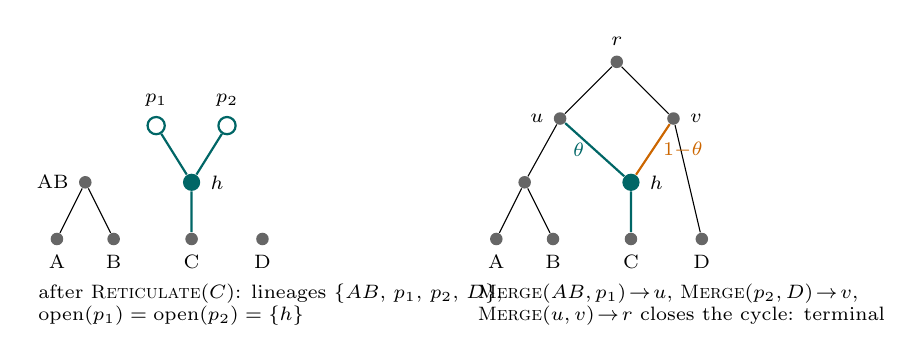
\begin{tikzpicture}[scale=0.9, every node/.style={font=\scriptsize}, dot/.style={circle,fill=black!60,inner sep=1.6pt}, ret/.style={circle,fill=teal!80!black,inner sep=2.2pt}, slot/.style={circle,draw=teal!80!black,thick,inner sep=2.2pt,fill=white}]
% state 2: reticulate C
\node[dot,label=below:A] (A) at (0,0) {}; \node[dot,label=below:B] (B) at (0.8,0) {}; \node[dot,label=below:C] (C) at (1.9,0) {}; \node[dot,label=below:D] (D) at (2.9,0) {};
\node[dot,label=left:AB] (AB) at (0.4,0.8) {}; \draw (AB)--(A) (AB)--(B);
\node[ret,label=right:$h$] (h) at (1.9,0.8) {}; \draw[teal!80!black,thick] (h)--(C);
\node[slot,label=above:$p_1$] (p1) at (1.4,1.6) {}; \node[slot,label=above:$p_2$] (p2) at (2.4,1.6) {};
\draw[teal!80!black,thick] (p1)--(h) (p2)--(h);
\node[align=left,anchor=north west] at (-0.4,-0.5) {after \textsc{Reticulate}$(C)$: lineages $\{AB,\,p_1,\,p_2,\,D\}$,\\ $\mathrm{open}(p_1)=\mathrm{open}(p_2)=\{h\}$};
% state 3
\begin{scope}[xshift=6.2cm]
\node[dot,label=below:A] (A) at (0,0) {}; \node[dot,label=below:B] (B) at (0.8,0) {}; \node[dot,label=below:C] (C) at (1.9,0) {}; \node[dot,label=below:D] (D) at (2.9,0) {};
\node[dot] (AB) at (0.4,0.8) {}; \draw (AB)--(A) (AB)--(B);
\node[ret,label=right:$h$] (h) at (1.9,0.8) {}; \draw[teal!80!black,thick] (h)--(C);
\node[dot,label=left:$u$] (u) at (0.9,1.7) {}; \draw (u)--(AB); \draw[teal!80!black,thick] (u)--(h) node[midway,left]{$\theta$};
\node[dot,label=right:$v$] (v) at (2.5,1.7) {}; \draw (v)--(D); \draw[orange!80!black,thick] (v)--(h) node[midway,right]{$1{-}\theta$};
\node[dot,label=above:$r$] (r) at (1.7,2.5) {}; \draw (r)--(u) (r)--(v);
\node[align=left,anchor=north west] at (-0.4,-0.5) {\textsc{Merge}$(AB,p_1)\!\to\!u$, \textsc{Merge}$(p_2,D)\!\to\!v$,\\ \textsc{Merge}$(u,v)\!\to\!r$ closes the cycle: terminal};
\end{scope}
\end{tikzpicture}
\end{center}

\paragraph{Trajectory length.} Each \textsc{Merge} removes one lineage, each \textsc{Reticulate} adds one; from $N$ lineages to $1$ with $R$ reticulations takes $N-1+R$ merges and $R$ reticulate actions: $N-1+2R$ steps (checked by \code{test\_trajectory\_length\_and\_reward}).

\subsection{The three masks and why there are no dead ends}
\begin{keybox}[Legality (constant time per action)]
\begin{itemize}[nosep]
\item \textsc{Merge}$(u,v)$ is legal iff $|\mathrm{open}(u)\cup\mathrm{open}(v)|\le1$ and $(u,v)$ are not the two bare slots of the same $h$.
\item \textsc{Reticulate}$(x)$ is legal iff $\mathrm{open}(x)=\emptyset$, fewer than $R_{\max}$ reticulations exist, and some \emph{other} lineage $y\neq x$ has $\mathrm{open}(y)=\emptyset$.
\end{itemize}
\end{keybox}
\emph{Why the first rule.} Merging two lineages that carry two different open reticulations $h\ne h'$ would create a node through which two cycles pass; in a binary network two cycles that share a vertex necessarily share an edge (a vertex of degree 3 cannot host two edge-disjoint cycles), which is level-2. Merging the two bare slots of one $h$ would create two parallel edges into $h$.

\emph{Why the second rule (no dead ends).} After \textsc{Reticulate}$(x)$ the slots $p_1,p_2$ cannot merge with each other and cannot merge with a lineage carrying a different open reticulation; they need a \emph{free} lineage ($\mathrm{open}=\emptyset$). The state $\{p_1,p_2,q_1,q_2\}$ (two bare pairs, nothing else) has no legal action at all. Requiring another free lineage at the moment of reticulating makes such states unreachable: by induction, every reachable non-terminal state has at least one legal action (if two free lineages exist, merge them; if one free and a pair, merge the free one into a slot; if only pairs, at least one pair is not bare, and its two carriers can close). The test \code{test\_class\_counts\_and\_no\_dead\_ends} enumerates \emph{all} reachable states for $N\le5$ and finds no dead end.

\emph{Why this is exactly the level-1 class.} Every terminal network is binary, acyclic (a new node is always older than what it connects) and level-1 (each cycle closes at exactly one reticulation and cycles are vertex-disjoint by the first rule). Conversely every level-1 network is reachable (induction on $R$: remove one cycle, build the rest, reticulate at the right moment). The enumeration in Part~VI confirms both directions numerically: the reachable terminal networks are $603=15+228+360$ for $N=4,R\le2$ and $11\,460=105+2\,805+8\,550$ for $N=5$, the published counts.

\subsection{Two features per lineage: the exact likelihood without $2^R$ trees}
\begin{keybox}[The trick]
A lineage $u$ that carries an open reticulation $h$ stores two Felsenstein features:
\begin{itemize}[nosep]
\item $A_u$ = feature of $u$ in the displayed trees where $u$'s side \emph{keeps} its edge into $h$;
\item $B_u$ = feature of $u$ in the displayed trees where that edge is \emph{deleted}.
\end{itemize}
For a bare slot: $A_{p_1}=\theta_h\,L_h$, $A_{p_2}=(1-\theta_h)\,L_h$, $B_{p_1}=B_{p_2}=\mathbf 1$ (all-ones: ``no data below'').\\
\textsc{Merge}$(u,v)\to w$ with lengths $(b_u,b_v)$, writing $T_u(\cdot)=(\cdot)\,P(b_u)^{\!\top}$:
{\small\begin{align*}
\text{both closed:}\ & A_w=T_u(A_u)\odot T_v(A_v);\\
\text{only $u$ open ($w$ stays open):}\ & A_w=T_u(A_u)\odot T_v(A_v),\quad B_w=T_u(B_u)\odot T_v(A_v);\\
\text{closing merge ($w$ closed):}\ & A_w=T_u(A_u)\odot T_v(B_v)+T_u(B_u)\odot T_v(A_v).
\end{align*}}
Edge priors $P(b)^{1/m}$ multiply both versions, exactly as in PhyloGFN.
\end{keybox}

\begin{proposition}\label{prop:mix}
For every level-1 network built by the MDP, the feature $A$ of the final lineage equals, at every site $i$, $\sum_{T\in\mathcal T(G)}w(T\mid\btheta)\,L^i_{\mathrm{root}}(\cdot\mid T,\bb)$ (times the edge priors). Hence $\sum_a\tfrac14A^i(a)$ is the network likelihood of site $i$ (eq.~\eqref{eq:netlik}).
\end{proposition}
\begin{proof}[Proof sketch]
Fix a reticulation $h$ with carriers $u$ (slot 1 side) and $v$ (slot 2 side) at the closing merge. The displayed trees split into those keeping $p_1$ (weight $\theta_h\cdot$rest) and those keeping $p_2$. In a tree keeping $p_1$, the edge $v\to h$ is deleted and the slot is suppressed, so $v$ contributes its feature \emph{without} the $h$ subtree: that is $B_v$ (the all-ones vector of a bare slot is invariant under $T_v$ because $P(b)\mathbf 1=\mathbf 1$, and suppressing a degree-2 node is exactly $P(b_1)P(b_2)=P(b_1+b_2)$). Symmetrically for trees keeping $p_2$. Because pruning is linear in each child feature and $\theta_h,1-\theta_h$ were folded into $A_{p_1},A_{p_2}$, the sum of the two products is the $\theta$-weighted sum over the two families of displayed trees. Cycles of a level-1 network are vertex-disjoint, so the families of different reticulations are independent and the argument applies to each closing merge in turn; nested (closed) cycles enter as already-mixed features, by linearity.
\end{proof}
The test \code{test\_likelihood\_matches\_explicit} compares this with an explicit enumeration of all $2^R$ displayed trees (\file{src/utils/network\_likelihood.py}) on random networks with up to 7 leaves and 3 reticulations; the largest difference is $1.5\times10^{-11}$.

\begin{whybox}[Why this matters for scalability]
The naive network likelihood costs $2^R$ Felsenstein passes; ours costs \emph{one} pass with at most two vectors per lineage --- $O(N\,m\,|\Sigma|^2)$ per trajectory, the same order as a tree. This is what makes reward evaluation compatible with the ``reward is the dominant per-trajectory cost'' analysis of the proposal.
\end{whybox}

\subsection{Ordering keys: keeping the list sorted so that actions are reproducible}
PhyloGFN sorts subtrees by their smallest leaf index. A bare slot has no leaves, and the leaves below $h$ would be counted by \emph{both} sides of $h$. We therefore give every lineage a set of \emph{tokens}: the leaf indices $0,\dots,N-1$, plus one fresh token $N+\mathrm{id}(h)$ for slot 2 of every reticulation; slot 1 inherits the tokens of $h$'s child. Tokens partition a set, so the minimum token (the \emph{key}) of each lineage is unique and the sorted-by-key list is well defined. \textsc{Merge}$(i<j)$ places the new lineage at position $i$; \textsc{Reticulate}$(i)$ places $p_1$ at position $i$ and appends $p_2$ (its fresh token is larger than every other key). The backward sampler recomputes action indices by replaying forward under this convention (\code{test\_backward\_sampling\_roundtrip}).

\subsection{Backward policy: counting parents correctly}
$|\mathrm{Pa}(s')|=$ (number of real lineages whose root is a tree node: undo a merge) $+$ (number of reticulations whose two slots are both bare in $s'$, \emph{provided $s'$ contains a free lineage}: undo a reticulation). The proviso is essential: undoing \textsc{Reticulate}$(x)$ leads to a state from which \textsc{Reticulate}$(x)$ is legal only if another free lineage exists; without the proviso we would count a ``parent'' that is not in the state graph, and $\PB$ would not be a distribution over actual parents --- the TB identity would be silently wrong. At the terminal state (rooted network) there is exactly one parent, the un-merge of the root; we keep the terminal object \emph{rooted} (reticulations are directed, so the root is meaningful), unlike PhyloGFN's unrooted trees with $2N-3$ last-step parents.

\subsection{Priors}
$p(\bb)=\prod_e\lambda e^{-\lambda b_e}$ with PhyloGFN's root convention (the two root edges count as one edge of length $b_l+b_r$); $p(\theta_h)=\mathrm{Uniform}(0,1)$. For the topology two priors are implemented (config \code{PRIOR\_TYPE}):
\begin{itemize}[nosep]
\item \code{EXP\_R} (the proposal's formula): $p(G)\propto e^{-\lambda_RR(G)}$ over the level-1 class, $R\le R_{\max}$;
\item \code{UNIFORM\_R}: $p(R)\propto e^{-\lambda_RR}$ and, given $R$, uniform over the $r(N,R)$ topologies: $\log p(G)=-\lambda_RR-\log r(N,R)+\text{const}$.
\end{itemize}
The difference is not cosmetic. The class sizes grow fast with $R$: for $N=6$, $r(6,1)/r(6,0)=41.6$ and $r(6,2)/r(6,1)=5.0$; for $N=27$ the ratios are in the thousands. Under \code{EXP\_R} the prior mass of ``some $R$'' is $r(N,R)e^{-\lambda_RR}$, so with $\lambda_R=1$ a 6-taxon prior already favours $R=2$ over $R=1$ by $1.8:1$ and $R=1$ over $R=0$ by $15:1$ \emph{before seeing any data}. \code{UNIFORM\_R} removes the class-size effect and makes $\lambda_R$ a genuine penalty per reticulation ($p(R)\propto e^{-\lambda_R R}$). Both are exact in the code; the normaliser needed for the MLL estimate uses the exact counts $r(N,k)$ in the first case and $\sum_k e^{-\lambda_Rk}$ in the second. Because $\log p(G)$ is added to $\log\R$, the sampler's marginal over $R$ is a genuine posterior over the number of reticulations under the chosen prior.

\subsection{The policy for two kinds of action}
The Transformer sees, per lineage, $[\,\bar A\,;\,\bar B\,;\,\text{4 flags}\,]$ where $\bar A,\bar B$ are the per-site normalised features (as PhyloGFN normalises $\rho$) and the flags are (has open reticulation, is bare slot, which side of $h$, its inheritance share $\theta$ or $1-\theta$). The flags let the policy recognise the two carriers of the same $h$ (their $A$ vectors share the $h$-subtree pattern). The action logits are the concatenation $[\text{pair logits}\mid\text{single logits}]$: pairs from the PhyloGFN head on $e_i+e_j$, singles from a new head on $e_i$; illegal entries are set to $-\infty$ using the environment's mask; $\varepsilon$-exploration picks a uniformly random \emph{legal} action. A \textsc{Reticulate} action then draws $(\log b_{hx},\mathrm{logit}\,\theta_h)$ from a 2-D Gaussian mixture (new head) with the change of variables $\log p(\theta)=\log p(\mathrm{logit}\,\theta)-\log\theta-\log(1-\theta)$.

\subsection{Variable-length batches}
Trajectories in a batch no longer share a step index, so the rollout worker keeps a \code{done} mask, runs the policy only on active trajectories, pads the lineage dimension to $l_{\max}=N+R_{\max}$ (the Transformer already supports padding masks) and accumulates $\sum\log\PF$ and $\sum\log\PB$ per trajectory as it goes. The TB loss is then identical in form to PhyloGFN's.
\clearpage

\section{Part V --- The modifications, one by one}

\noindent\textbf{Principle.} The original files are left untouched except for four small \emph{registrations} (M12). Every new behaviour lives in new files whose names end in \code{\_net} or \code{network}, so that \code{git diff} shows exactly what was added and the tree sampler keeps working unchanged (\code{ENVIRONMENT\_TYPE: ONE\_STEP\_BINARY\_TREE}). Table~\ref{tab:mods} is the map.

\begin{table}[h]\centering\small
\begin{tabular}{lp{7.2cm}p{5.6cm}}\toprule
\textbf{Id} & \textbf{File (new unless marked)} & \textbf{Content} \\ \midrule
M1 & \pfile{src/env/phylo_network_env.py} & node / lineage / state / network data structures \\
M2 & \pfile{src/env/phylo_network_env.py} & initial state and the two-version feature tensor \\
M3 & \pfile{src/env/phylo_network_env.py} & level-1 masks \\
M4 & \pfile{src/env/phylo_network_env.py} & transitions \textsc{Merge} / \textsc{Reticulate}, ordering keys \\
M5 & \pfile{src/env/phylo_network_env.py} & feature updates = exact likelihood, reward \\
M6 & \pfile{src/env/phylo_network_env.py} & number of parents, backward sampling from a network \\
M7 & \pfile{src/env/phylo_network_env.py} & policy inputs: normalisation, flags, masks, padding \\
M8 & \pfile{src/model/network_model/one_step_network_model.py}, \pfile{src/model/edges_model/continuous/network_heads.py} & policy with two action types; heads for lengths and $\theta$ \\
M9 & \pfile{src/utils/level1_counts.py} & exact class sizes; topology prior normaliser \\
M10 & \pfile{src/gfn/tb_gfn_net.py} & generator: routing of actions, TB loss \\
M11 & \pfile{src/gfn/rollout_worker_net.py}, \pfile{src/gfn/training_data_loader_net.py}, \pfile{src/gfn/gfn_evaluator_net.py} & variable-length rollouts, replay buffer, evaluation \\
M12 & \pfile{src/configs/defaults.py}, \pfile{src/env/__init__.py}, \pfile{src/gfn/build.py}, \pfile{src/utils/utils.py} (modified); \pfile{train_net.py}, \pfile{src/configs/network_cfgs/*.yaml}, \pfile{tools/*}, \pfile{tests/*} & registrations, config, training script, data simulation, tests \\
\bottomrule
\end{tabular}
\caption{Where each modification lives.}\label{tab:mods}
\end{table}

% ---------------------------------------------------------------------------
\subsection{M1 --- Data structures: nodes with two parents}
\textbf{What.} PhyloGFN stores trees as \code{ete3.TreeNode}, which has exactly one parent per node. A reticulation node needs two. \code{NetNode} is a minimal DAG node; \code{Lineage} is an entry of the state list (a real root, or a bare slot); \code{NetworkState} replaces \code{PhylogenticTreeState}; \code{PhyloNetwork} replaces \code{PhylogeneticTree} (same interface: \code{log\_score}, \code{signature}, ordering for the replay heap).
\begin{lstlisting}
class NetNode(object):
    """kind: 'leaf' | 'tree' | 'ret'
       ret: one child (child_dist), two parents = two SLOTS parents[k], parent_dists[k];
            theta = inheritance weight of slot 0, 1 - theta of slot 1."""
    __slots__ = ('idx', 'kind', 'children', 'child_dists', 'parents', 'parent_dists',
                 'theta', 'child_dist', 'tokens', 'ret_id')

class Lineage(object):
    """node: NetNode; slot: None (real lineage) or 0/1 (bare parent slot of node = h);
       open_h: the unclosed reticulation carried (None if closed);
       tokens: ownership tokens; key = min(tokens) (unique -> sorted state list)."""

class NetworkState(object):
    def __init__(self, lineages, next_idx, n_ret, log_reward=None, log_score=None):
        self.lineages = lineages; self.next_idx = next_idx; self.n_ret = n_ret
        self.is_done = (len(lineages) == 1 and lineages[0].open_h is None)
\end{lstlisting}
\textbf{Why.} Everything downstream (transitions, likelihood, backward sampling, canonical signatures) needs to know, for a reticulation, \emph{which} parent is which and what $\theta$ belongs to which slot. \code{network\_canonical\_string} writes a reticulation subtree as \code{\#<subtree>} at both parent positions; on level-1 networks with labelled leaves this string is a faithful topology identifier (used by the replay buffer instead of ete3's \code{get\_topology\_id}).

% ---------------------------------------------------------------------------
\subsection{M2 --- Initial state and the feature tensor}
\textbf{What.} \code{get\_initial\_state} creates $N$ leaf lineages with token sets $\{0\},\dots,\{N-1\}$. \code{initial\_features(B)} returns a tensor of shape $[B,\,l_{\max},\,2,\,m,\,4]$ (two versions per lineage) filled with ones, with the one-hot sequences copied into \emph{both} versions of the first $N$ rows.
\begin{lstlisting}
self.l_max = self.n_leaves + self.r_max            # a RETICULATE adds one lineage
rows, cols = torch.triu_indices(self.l_max, self.l_max, offset=1)
self.n_pairs = len(rows);  self.n_actions = self.n_pairs + self.l_max   # [pairs | singles]

def initial_features(self, batch):
    feats = torch.ones(batch, self.l_max, 2, self.m, self.c, dtype=..., device=...)
    feats[:, :self.n_leaves, 0] = self.seq_arrays
    feats[:, :self.n_leaves, 1] = self.seq_arrays
    return feats
\end{lstlisting}
\textbf{Why.} PhyloGFN's tensor is $[B,l,m,4]$ with $l$ shrinking by one every step for \emph{all} trajectories. Ours must (i) hold two versions and (ii) keep a fixed width $l_{\max}=N+R_{\max}$ because the number of lineages differs between trajectories of the same batch; unused rows are ones and are hidden from the policy by a padding mask (M7). The action space is laid out once, over $l_{\max}$: pair $k\mapsto(\code{rows}[k],\code{cols}[k])$, single $n_{\text{pairs}}+i\mapsto$ lineage $i$.

% ---------------------------------------------------------------------------
\subsection{M3 --- Level-1 masks}
\textbf{What.} \code{legal\_actions(state)} returns a boolean vector over the padded action space; \code{merge\_legal(u,v)} is the pair rule.
\begin{lstlisting}
def legal_actions(self, state):
    L = state.lineages; n = len(L)
    mask = np.zeros(self.n_actions, dtype=bool)
    if state.is_done: return mask
    for i in range(n):
        for j in range(i + 1, n):
            mask[self.pair_index[(i, j)]] = self.merge_legal(L[i], L[j])
    n_free = sum(1 for l in L if l.open_h is None)
    if state.n_ret < self.r_max:
        for i in range(n):
            if L[i].open_h is None and n_free >= 2:     # x free AND another free lineage exists
                mask[self.n_pairs + i] = True
    return mask

@staticmethod
def merge_legal(u, v):
    if u.open_h is not None and v.open_h is not None:
        if u.open_h is not v.open_h: return False     # two different open cycles: level-2
        if u.is_bare and v.is_bare:  return False     # the two bare slots of one h: parallel edges
    return True
\end{lstlisting}
\textbf{Why.} See Part~IV.2. The three rules are $O(1)$ per candidate action because $\mathrm{open}(u)$ is stored on the lineage, never recomputed from the graph. In PhyloGFN every pair is legal, so the only mask is the padding mask; here the mask is also the definition of the class.

% ---------------------------------------------------------------------------
\subsection{M4 --- Transitions and ordering keys}
\textbf{What.} \code{apply\_action(state, action, feats)} implements both actions on the Python state and (optionally) on the feature tensor; it returns \code{(new\_state, new\_feats, log\_score)} with \code{log\_score} set only at a terminal state. The \textsc{Merge} branch is PhyloGFN's \code{update\_state} plus the slot bookkeeping; the \textsc{Reticulate} branch is new.
\begin{lstlisting}
# MERGE(i, j): new tree node w; a bare slot attaches the reticulation node itself
for lin, d, slot_side in ((u, bl, 0), (v, br, 1)):
    child = lin.node
    w.children.append(child); w.child_dists.append(d)
    if lin.is_bare:                                # fill the slot: edge w -> h of length d
        child.parents[lin.slot] = w; child.parent_dists[lin.slot] = d
open_h = None if case in (0, 3) else (u.open_h if case == 1 else v.open_h)
new_lin = Lineage(w, open_h=open_h, tokens=u.tokens | v.tokens)
new_L = L[:i] + [new_lin] + L[i + 1:j] + L[j + 1:]      # result at position i, j removed

# RETICULATE(i): h above lineage x, two bare slots p1 (position i) and p2 (appended)
h = NetNode(state.next_idx, 'ret'); h.children = [x.node]; h.child_dist = b_hx; h.theta = theta
fresh = self.n_leaves + state.n_ret                     # ordering token of slot 1
p1 = Lineage(h, slot=0, open_h=h, tokens=x.tokens)
p2 = Lineage(h, slot=1, open_h=h, tokens=[fresh])
new_L = L[:i] + [p1] + L[i + 1:] + [p2]
\end{lstlisting}
\textbf{Why.} \code{case} (0 both closed, 1 only $u$ open, 2 only $v$ open, 3 closing) decides both the open status of the result and the feature rule (M5). The token discipline replaces \code{min\_seq\_idx}: keys are unique and the list stays sorted, which is what the backward sampler needs to reconstruct the same action indices (Part~IV.4).

% ---------------------------------------------------------------------------
\subsection{M5 --- Feature updates: the exact likelihood and the reward}
\textbf{What.} Three private methods replace \code{compute\_partial\_prob}'s role for networks.
\begin{lstlisting}
def _merge_features(self, feats, i, j, case, bl, br, last_step):
    uA, uB = feats[i, 0], feats[i, 1];  vA, vB = feats[j, 0], feats[j, 1]
    M = self.evolution_model.get_transition_matrices(torch.tensor([bl, br]))
    if last_step:      # PhyloGFN root convention: one prior on b_l + b_r (pulley principle)
        tu = lambda f: f @ M[0]; tv = lambda f: f @ M[1]; prior = exp(log_prior(bl + br) / m)
    else:              # edge priors folded into the features, site by site (paper eq. 4)
        pl = exp(log_prior([bl, br]) / m)
        tu = lambda f: (f @ M[0]) * pl[0]; tv = lambda f: (f @ M[1]) * pl[1]; prior = 1.0
    if case == 0:   wA = tu(uA) * tv(vA) * prior;                 wB = wA
    elif case == 1: wA = tu(uA) * tv(vA) * prior;                 wB = tu(uB) * tv(vA) * prior
    elif case == 2: wA = tu(uA) * tv(vA) * prior;                 wB = tu(uA) * tv(vB) * prior
    else:           wA = (tu(uA) * tv(vB) + tu(uB) * tv(vA)) * prior;  wB = wA   # closing merge
    ... row j removed, row i <- (wA, wB), a row of ones appended to keep l_max rows

def _reticulate_features(self, feats, i, n, theta, b_hx):
    Lh = self._transport(feats[i, 0][None], torch.tensor([b_hx]))[0]   # M(b_hx) L_x * prior^(1/m)
    new[i, 0] = theta * Lh;        new[i, 1] = ones          # slot 0 at position i
    new[n, 0] = (1 - theta) * Lh;  new[n, 1] = ones          # slot 1 appended at position n

def log_topology_prior_unnormalised(self, n_ret):
    if self.prior_type == 'UNIFORM_R':                                   # p(R) ~ exp(-λR), uniform within R
        return -self.lambda_r * n_ret - self.log_class_size[n_ret]
    return -self.lambda_r * n_ret                                        # EXP_R: p(G) ~ exp(-λR) over the class

def _terminal_log_score(self, root_feat, n_ret):
    log_p = torch.sum(torch.log(torch.sum(root_feat / 4.0, -1)), -1)   # sum_i log sum_a A^i(a)/4
    return float(log_p) + self.log_topology_prior_unnormalised(n_ret)   # + log p(G)
\end{lstlisting}
\textbf{Why.} This is Proposition~\ref{prop:mix} in code. Note what did \emph{not} change: the transition matrices, the edge prior, the per-site folding of $P(b)^{1/m}$, the root formula $\sum_i\log\sum_a L^i(a)/4$ and the last-step convention are all PhyloGFN's --- with $R_{\max}=0$ the code computes exactly PhyloGFN's reward (Part~VI.4). The reward reshaping \code{(C + log\_score)/scale} is reused from \code{PhyloTreeReward}.

% ---------------------------------------------------------------------------
\subsection{M6 --- Backward policy: counting parents, sampling backward}
\textbf{What.} \code{NetworkState.num\_parents()} and \code{PhyloNetworkEnv.sample\_backward\_from\_network(net)}.
\begin{lstlisting}
def num_parents(self):
    n = 0; seen_ret = {}; n_free = 0
    for l in self.lineages:
        if l.is_bare: seen_ret[l.node.idx] = seen_ret.get(l.node.idx, 0) + 1
        else:
            if l.open_h is None: n_free += 1
            if l.node.kind == 'tree': n += 1                   # un-merge
    if n_free >= 1:
        n += sum(1 for c in seen_ret.values() if c == 2)       # un-reticulate (only if legal forward)
    return n
\end{lstlisting}
\code{sample\_backward\_from\_network} walks backward from the finished network: at every step it lists the undo moves (un-merge any tree-root lineage; un-reticulate any $h$ whose two slots are both bare, provided a free lineage exists), records their number ($=|\mathrm{Pa}|$), picks one uniformly, and stops at the leaves. It then \emph{replays forward}, matching the original nodes to freshly created ones (\code{new\_of}) to recover the pair / lineage indices under the sorted convention, and attaches the stored lengths and $\theta$'s. It returns \code{(actions, log\_paths\_pb)} exactly like \code{sample\_backward\_from\_tree}.\\
\textbf{Why.} Uniform $\PB$ requires the true number of parents in the state graph (Part~IV.5); the replay-buffer training and the Pearson-$r$ evaluation both need backward-sampled trajectories of a \emph{given} network. \code{test\_backward\_sampling\_roundtrip} checks that the replay yields the same canonical network, the same score and the same $|\mathrm{Pa}|$ sequence as the forward code.

% ---------------------------------------------------------------------------
\subsection{M7 --- What the policy sees}
\textbf{What.} \code{prepare\_rollout\_inputs(feats, states, random\_spec, input\_actions)} normalises both versions per site (as PhyloGFN's \code{NORMALIZE\_LIKELIHOOD}), flattens them, appends four flags per lineage, and returns the padding mask, the action mask and the pair index tables.
\begin{lstlisting}
x = feats / feats.sum(-1, keepdim=True); x[isnan] = 1/4          # per-site normalisation of A and B
x = x.reshape(b, self.l_max, -1)                                  # [b, l_max, 2*m*4]
flags[k, i] = [has_open, is_bare, side (slot 0 / slot 1), share (theta or 1 - theta)]
x = torch.cat([x, flags], dim=-1)
pad = torch.arange(self.l_max)[None] >= nb[:, None]               # True = padding
masks[k] = self.legal_actions(s)                                  # True = legal
\end{lstlisting}
\textbf{Why.} The Transformer needs a set of fixed-size vectors; padding rows are excluded by \code{key\_padding\_mask}, illegal actions by the action mask. The flags give the policy the information the masks use (Part~IV.7); the environment --- not the network --- remains the single authority on legality.

% ---------------------------------------------------------------------------
\subsection{M8 --- The policy and the two continuous heads}
\textbf{What.} \code{PhyloNetworkModelOneStep} keeps PhyloGFN's encoder and pair head and adds \code{single\_logits\_head}; \code{MergeEdgeModel} serves root-mode and two-edge-mode merges in one batch; \code{ReticulationModel} samples $(\log b_{hx},\mathrm{logit}\,\theta)$.
\begin{lstlisting}
pairs   = reps[:, rows] + reps[:, cols]                    # e_i + e_j   (PhyloGFN)
singles = reps                                             # e_i         (new)
pair_logits   = self.pair_logits_head(cat[pairs, summary]).squeeze(-1)
single_logits = self.single_logits_head(cat[singles, summary]).squeeze(-1)
logits = torch.cat([pair_logits, single_logits], dim=1).masked_fill(~action_mask, -inf)
actions = self.sample(logits, action_mask, random_spec)   # epsilon-greedy over LEGAL actions
log_paths_pf = log_softmax(logits)[arange(B), actions]
\end{lstlisting}
\begin{lstlisting}
class ReticulationModel(nn.Module):        # 2-D diagonal Gaussian mixture over (log b_hx, logit theta)
    def forward(self, summary_reps, lineage_reps, input_ret_actions=None):
        dist = self.distribution(torch.cat([summary_reps, lineage_reps], 1))
        z = dist.sample();  z = [z0.clip(-10, 0), z1.clip(-r-2, r+2)]
        lp = dist.log_prob(z)
        b_hx, theta = exp(z0), sigmoid(z1)
        lp = lp - z0 - log(theta) - log(1 - theta)          # change of variables for b and theta
        return b_hx, theta, lp
\end{lstlisting}
\textbf{Why.} The discrete choice and the continuous draw are two factors of one transition density; TB needs $\log\PF$ of the \emph{whole} step, so the head's log-density (with the Jacobian terms) is added to the discrete log-probability in the generator (M10). Squashing the mean of $\log b$ into $[-10,0]$ is PhyloGFN's trick (App.~F); the analogous squash of $\mathrm{logit}\,\theta$ into $[-6,6]$ keeps $\theta$ away from the numerically degenerate ends $0$ and $1$ at initialisation.

% ---------------------------------------------------------------------------
\subsection{M9 --- Exact class sizes and the topology prior}
\textbf{What.} \file{level1\_counts.py} implements the closed formula of Bouvel, Gambette \& Mansouri (2020, Prop.~5.4) for $r(n,k)$, the number of rooted binary level-1 networks with $n$ labelled leaves and $k$ reticulations, and the prior normaliser $\log Z_\lambda=\log\sum_{k\le R_{\max}}r(n,k)e^{-\lambda_Rk}$ (\code{EXP\_R}) or $\log\sum_{k\le R_{\max}}e^{-\lambda_Rk}$ (\code{UNIFORM\_R}); the environment also uses $\log r(N,R)$ in the reward under \code{UNIFORM\_R}.
\begin{lstlisting}
def log_topology_prior_normalizer(n, r_max, lambda_r):
    terms = [log(level1_count(n, k)) - lambda_r * k for k in range(0, r_max + 1)]
    mx = max(terms);  return mx + log(sum(exp(t - mx) for t in terms))
\end{lstlisting}
\textbf{Why.} It is the network analogue of PhyloGFN's \code{tree\_factor} $=-\log(2N-5)!!$ in the MLL estimator: without it the ``MLL'' would be off by the log of the prior normaliser. The formula was checked against the paper's Table~2 totals (36, 723, 20\,280, 730\,755) and against our own enumeration for $N\le6$; exact integers, no floating point.

% ---------------------------------------------------------------------------
\subsection{M10 --- The generator}
\textbf{What.} \code{TBGFlowNetNet.forward(input\_dict)} runs the policy, then routes the sampled ids: merges go to \code{MergeEdgeModel}, reticulations to \code{ReticulationModel}; the log-densities are added with \code{index\_add}; the environment-format action dicts are assembled. Replay trajectories arrive as \code{input\_actions} (one dict or \code{None} per trajectory) and are converted into forced ids and forced parameters (\code{nan} = not forced).
\begin{lstlisting}
is_merge = actions < env.n_pairs
sel = where(is_merge);  edges, lp = self.edges_model(summary[sel], left, right, last_step[sel], edge_given[sel])
log_pf = log_pf.index_add(0, sel, lp)
sel = where(~is_merge); b_hx, theta, lp = self.ret_model(summary[sel], reps[sel, lineage], ret_given[sel])
log_pf = log_pf.index_add(0, sel, lp)
# loss (unchanged form):  ( log Z + log_pf  -  log_reward - log_pb )^2
\end{lstlisting}
\textbf{Why.} PhyloGFN's generator always calls the edge model for \emph{every} row of the batch; ours must split rows by action type. The TB loss, $\log Z$ parametrisation (256-vector), optimiser groups, gradient clipping and temperature rescaling are copied unchanged.

% ---------------------------------------------------------------------------
\subsection{M11 --- Rollouts, replay buffer, evaluation}
\textbf{Rollout worker.}
\begin{lstlisting}
done = np.array([s.is_done for s in states])
while not done.all():
    active = np.where(~done)[0]
    input_dict = env.prepare_rollout_inputs(feats[active], act_states, random_spec, input_actions)
    ret = generator(input_dict)
    new_states, new_feats, ls, lr = env.batch_apply_actions(ret['actions'], feats[active], act_states)
    feats[active] = new_feats
    log_pf = log_pf.index_add(0, active, ret['log_paths_pf'])
    log_pb = log_pb.index_add(0, active, -log(tensor([s.num_parents() for s in new_states])))
    ... mark finished trajectories, store log_rewards / log_scores / n_ret
\end{lstlisting}
\textbf{Why.} Lock-step batching (\code{while tree\_features.shape[1] > 1}) is impossible with variable lengths; the \code{done} mask and per-trajectory accumulation are the minimal change. The parent count of the \emph{new} state is used, as in PhyloGFN; the last step now has one parent instead of $2N-3$ (rooted terminal object).\\
\textbf{Replay buffer} (\file{training\_data\_loader\_net.py}): same heap logic, keyed by the canonical network signature; backward trajectories from \code{sample\_backward\_from\_network}.\\
\textbf{Evaluator} (\file{gfn\_evaluator\_net.py}): eq.~\eqref{eq:mll} with $-\log Z_\lambda$ from M9, plus the histogram of sampled $R$ (the posterior over the number of reticulations) --- the quantity the validation plan calls ``posterior mode $R$'' (T8).

% ---------------------------------------------------------------------------
\subsection{M12 --- Registrations, configuration, scripts, tests}
\textbf{Modified original files (the entire diff to the original code).}
\begin{lstlisting}
# src/env/__init__.py
if cfg.ENV.ENVIRONMENT_TYPE == 'ONE_STEP_LEVEL1_NETWORK': env = PhyloNetworkEnv(cfg, all_seqs)
# src/gfn/build.py
if cfg.ENV.ENVIRONMENT_TYPE == 'ONE_STEP_LEVEL1_NETWORK': generator = TBGFlowNetNet(cfg.GFN, env, device, ddp)
# src/utils/utils.py  (correct_cfg_data): input size of the policy embedding
cfg.GFN.MODEL.TRANSFORMER.SEQ_EMB.INPUT_SIZE = 2 * seq_length * vocab_size + 4
# src/configs/defaults.py: ENV.NETWORK.{R_MAX, LAMBDA_R, PRIOR_TYPE}, TRANSFORMER.SINGLE_LOGITS_HEAD, RETICULATION_MODELING
\end{lstlisting}
\textbf{New scripts.} \pfile{train_net.py} (training loop without DDP/AMP; same schedules), \pfile{src/configs/network_cfgs/cfg_net_small_cpu.yaml} (a CPU-sized configuration), \pfile{tools/simulate_network_data.py} (alignments simulated on a known level-1 network; writes the truth), \pfile{tools/compare_tree_mode.py} ($R_{\max}=0$ versus PhyloGFN), \pfile{tests/test_network_env.py} (Part~VI).
\clearpage

\section{Part VI --- Verification: what was tested and what the tests showed}

\begin{keybox}[The standard]
A modification of a sampler is only worth presenting if (a) the object class is exactly the intended one, (b) the reward is exactly the intended likelihood, (c) the backward policy is exactly a distribution over parents, and (d) the whole thing reduces to the original when the new feature is switched off. Each of the four has an executable test.
\end{keybox}

\subsection{(a) The class: exhaustive enumeration of the MDP}
\file{tests/test\_network\_env.py::test\_class\_counts\_and\_no\_dead\_ends} runs a depth-first search over \emph{all} states reachable from $s_0$ (continuous values ignored; states memoised by a canonical string), collects the terminal networks by canonical string, and checks that every non-terminal state has at least one legal action.
\begin{center}\small
\begin{tabular}{ccrrr}\toprule
$N$ & $R_{\max}$ & reachable terminal networks & expected (Bouvel et al.\ 2020) & distinct states visited \\ \midrule
3 & 2 & 36 & 36 & 205 \\
4 & 1 & 243 & 243 & 1\,001 \\
4 & 2 & 603 & 603 & 4\,829 \\
5 & 1 & 2\,910 & 2\,910 & 12\,821 \\
5 & 2 & 11\,460 & 11\,460 & 109\,131 \\
\bottomrule
\end{tabular}
\end{center}
Dead ends: 0 in every case. The expected numbers are $\sum_{k\le R_{\max}}r(N,k)$ with $r(4,\cdot)=15,228,360$ and $r(5,\cdot)=105,2805,8550$; they were obtained from the published generating function and, independently, from a direct enumeration by insertion (\file{enum\_level1.py}, shipped with the validation material). Three different constructions agreeing on five numbers is as close to a proof-by-computer as this question allows.

\subsection{(b) The likelihood: two vectors versus $2^R$ displayed trees}
\file{src/utils/network\_likelihood.py} is a deliberately slow, independent implementation of eq.~\eqref{eq:netlik}: it enumerates the $2^R$ displayed trees, suppresses degree-2 nodes summing lengths, runs a plain \code{numpy} Felsenstein pass on each, mixes per site, and adds the same edge priors and the reticulation prior. \code{test\_likelihood\_matches\_explicit} draws random networks (random legal actions, random lengths and $\theta$) with $(N,R_{\max})\in\{(4,1),(5,2),(6,3),(7,2)\}$ and compares. Largest absolute difference over 48 networks: $1.5\times10^{-11}$ on log-scores of order $10^3$ --- floating-point agreement.

\subsection{(c) The backward policy}
\code{test\_backward\_sampling\_roundtrip}: for random terminal networks ($N=5,6,8$; $R\le3$), \code{sample\_backward\_from\_network} produces an action list of length $N-1+2R$; replaying it forward reproduces the same canonical network, the same log-score (to $10^{-6}$) and the same sequence of parent counts $|\mathrm{Pa}(s_t)|$ as \code{NetworkState.num\_parents()} computed on the forward states. This is the consistency that trajectory balance relies on.

\subsection{(d) Reduction to PhyloGFN}
With \code{R\_MAX: 0} the environment can only merge; the reward is PhyloGFN's; the policy has the same encoder and pair head (the single head is masked out). \file{tools/compare\_tree\_mode.py} trains the original implementation and the network implementation on the same 6-taxon, 300-site alignment with the same tiny budget (8 epochs $\times$ 40 steps $\times$ 48 trajectories, CPU) and estimates the evidence five times each:
\begin{center}\small
\begin{tabular}{lcc}\toprule
 & MLL (mean $\pm$ s.d.\ of 5 estimates) & wall-clock \\ \midrule
PhyloGFN (original code, \code{ONE\_STEP\_BINARY\_TREE}) & $-1838.92\pm0.38$ & 38 s \\
PhyloGFN-Net with $R_{\max}=0$ & $-1840.97\pm0.29$ & 91 s \\
\bottomrule
\end{tabular}
\end{center}
Both numbers are lower bounds of the same $\log P(\bY)$ (rooted and unrooted uniform priors give the same evidence under a reversible model); the two-unit gap at this budget is training noise (the network code trains fewer effective updates per second, Part~VIII.1). The check that matters is qualitative: the new code path is a functioning PhyloGFN when reticulations are disabled.

\subsection{(e) Learning on simulated data, and the negative control}
\file{tools/simulate\_network\_data.py} generated two 6-taxon, 300-site alignments with the same seed: one on a level-1 network with one reticulation ($\theta=0.5$), one on a tree. Four CPU runs of \file{train\_net.py} ($R_{\max}=2$, batch 48, temperature $8\to1$, $\varepsilon$ $0.5\to0.01$, 12--20 epochs of 40 steps, 10--20 minutes each) are summarised in Fig.~\ref{fig:runs}.

\begin{figure}[h]\centering
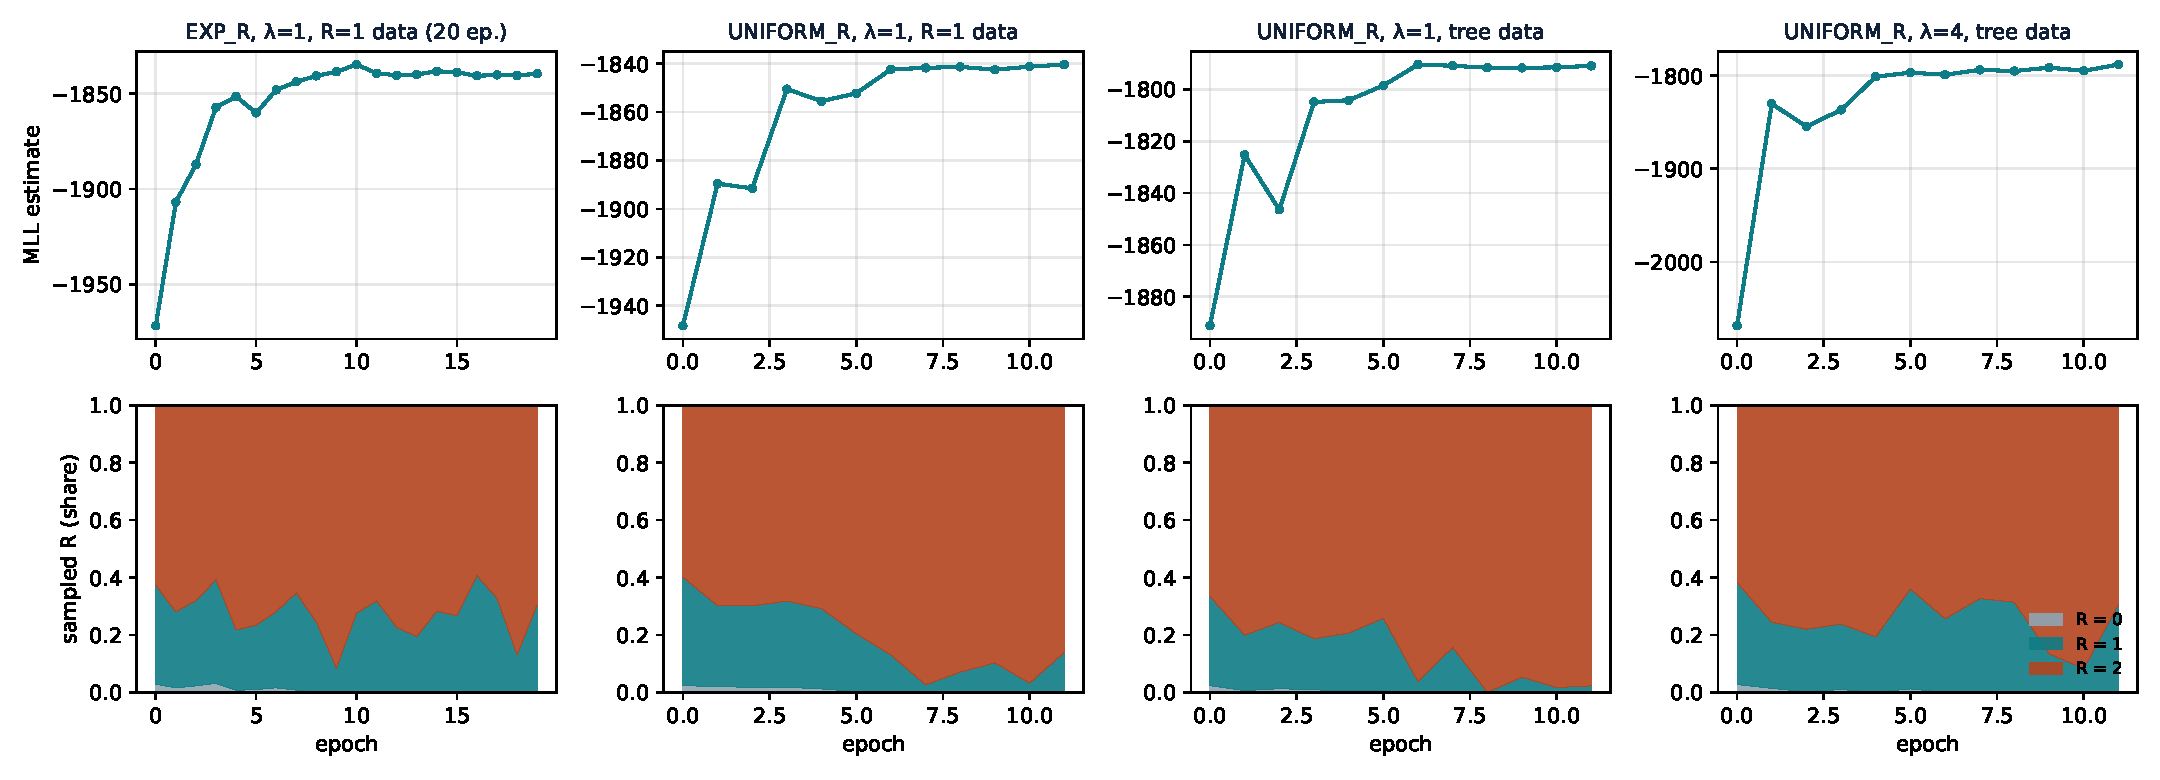
\includegraphics[width=\textwidth]{fig_runs.pdf}
\caption{Top: importance-weighted MLL estimate per epoch. Bottom: share of sampled networks with $R=0,1,2$ reticulations (1\,024 samples per epoch). Left to right: \code{EXP\_R} prior, $\lambda_R=1$, data with one reticulation; \code{UNIFORM\_R}, $\lambda_R=1$, same data; \code{UNIFORM\_R}, $\lambda_R=1$, tree-only data; \code{UNIFORM\_R}, $\lambda_R=4$, tree-only data.}\label{fig:runs}
\end{figure}

\begin{center}\small
\begin{tabular}{llccc}\toprule
data & prior & final MLL & sampled $R$ ($0/1/2$, last epoch) & Pearson $r$ \\ \midrule
$R=1$ & \code{EXP\_R}, $\lambda_R=1$ (20 ep.) & $-1840.6\pm0.6$ & 2 / 310 / 712 & 0.67 \\
$R=1$ & \code{UNIFORM\_R}, $\lambda_R=1$ & $-1842.2\pm0.4$ & 0 / 143 / 881 & 0.55 \\
tree & \code{UNIFORM\_R}, $\lambda_R=1$ & $-1789.8\pm1.5$ & 0 / 24 / 1000 & 0.51 \\
tree & \code{UNIFORM\_R}, $\lambda_R=4$ & $-1792.4\pm0.4$ & 1 / 313 / 710 & 0.65 \\
\bottomrule
\end{tabular}
\end{center}

\paragraph{What works.} The machinery trains: the bound rises by 100--180 log-units during the temperature anneal and then stabilises; the replay buffer fills with high-scoring networks; the two priors and $R_{\max}$ behave as configured; the reduction to PhyloGFN holds.

\paragraph{What does not work yet --- and why it is the right thing to have found.} The negative control (T8 of the validation plan: tree-only data must give posterior mode $R=0$) \emph{fails at this budget}: on tree-simulated data the sampler still returns $R=2$ for 70--98\,\% of its samples, with either prior and even with $\lambda_R=4$. The replay buffers contain no tree at all. The diagnosis is quantitative:
\begin{itemize}[nosep]
\item the true tree with re-optimised branch lengths scores $\log P(\bY\mid G,\bb)+\log P(\bb)=-1757.7$ on the tree data; the best $R=2$ network in the $\lambda_R=4$ buffer scores $-1746.3$ before the topology prior: \emph{12 nats higher};
\item six extra edges ($3R$) with lengths near zero each contribute up to $\log\lambda=\log10=2.3$ nats of prior \emph{density}: the reward is a density over $(G,\bb,\btheta)$ and adding dimensions adds density peaks. The posterior over $R$ is the \emph{integral} of that density over the extra dimensions (an Occam factor that removes the effect), and a converged GFlowNet reproduces the integral. A sampler trained for minutes, with a temperature schedule that first flattens the reward (where the far larger $R=2$ class dominates by volume) and a buffer that stores density peaks, inherits the preference for $R=2$. Pearson $r\approx0.5$--$0.7$ confirms that the fit is still coarse (PhyloGFN reaches $0.99$ after 500 epochs of 1\,000 steps).
\end{itemize}
This is exactly the situation the proposal's validation plan is designed to detect: the exact posterior at $N\le5$ (11\,460 topologies, O3) separates sampler error from prior behaviour; the negative control T8 must pass before any network claim. The prototype delivers the instrument; the remedies are on the roadmap (Part~VIII): longer training with the paper's schedule, the hyper-prior on $\lambda_R$ (or \code{UNIFORM\_R} with $\lambda_R$ set from the exact small-$N$ posterior), and a prior on reticulation edges that does not reward vanishing lengths.
\clearpage

\section{Part VII --- How to run everything}

\subsection{Installation}
\begin{lstlisting}[style=sh]
conda create -n phylogfn python=3.10 && conda activate phylogfn
pip install torch numpy scipy tqdm dill docopt fvcore ete3 networkx     # networkx: tests / data simulation only
\end{lstlisting}
(The original \code{README} lists the same packages via conda; \code{tensorboard} is only needed by the original \file{train.py}.)

\subsection{Run the verification tests first}
\begin{lstlisting}[style=sh]
python tests/test_network_env.py            # ~ 3-4 minutes on a laptop CPU
\end{lstlisting}
Expected output (abridged):
\begin{lstlisting}[style=sh]
N=4 R_MAX=2: reachable terminal networks 603 (expected 603); 4829 distinct states; dead ends 0
N=5 R_MAX=2: reachable terminal networks 11460 (expected 11460); 109131 distinct states; dead ends 0
max |fast - explicit| = 1.47e-11
backward round trip ok
trajectory lengths ok
ALL TESTS PASSED
\end{lstlisting}

\subsection{Simulate data with a known network and train}
\begin{lstlisting}[style=sh]
python tools/simulate_network_data.py dataset/simulated/sim6_r1.pickle --leaves=6 --sites=300 --rets=1 --seed=3
python train_net.py src/configs/network_cfgs/cfg_net_small_cpu.yaml dataset/simulated/sim6_r1.pickle runs/sim6_r1
\end{lstlisting}
The truth (edges, reticulation, $\theta$) is written to \file{dataset/simulated/sim6\_r1.truth.txt}. Each epoch prints the MLL estimate, the Pearson correlation and the histogram of the number of reticulations in 1\,024 samples; \file{runs/.../history.pkl} keeps them; \file{best\_networks.pt} is the replay buffer (a heap of \code{PhyloNetwork} objects, each with \code{.root}, \code{.log\_score}, \code{.topology\_id}).

\subsection{Train on a benchmark alignment}
\begin{lstlisting}[style=sh]
python train_net.py src/configs/network_cfgs/cfg_net_small_cpu.yaml dataset/benchmark_datasets/DS1.pickle runs/ds1_net --device=cuda
\end{lstlisting}
For DS1 ($N=27$) use a GPU and the PhyloGFN-sized architecture (\code{DEPTH: 6}, embedding 128, 500 epochs $\times$ 1\,000 steps as in \file{cfg\_continuous\_temperature\_anneal\_0.4.yaml}); the network config only changes \code{ENVIRONMENT\_TYPE}, \code{NETWORK.R\_MAX}, \code{NETWORK.LAMBDA\_R} and the two new heads.

\subsection{Tree mode (the equivalence check)}
\begin{lstlisting}[style=sh]
python tools/compare_tree_mode.py dataset/simulated/sim6_r1.pickle 8 40
\end{lstlisting}

\subsection{Configuration keys added}
\begin{center}\small
\begin{tabular}{p{5.6cm}p{2.6cm}p{6.3cm}}\toprule
Key & Default & Meaning \\ \midrule
\pfile{ENV.ENVIRONMENT_TYPE} & \pfile{ONE_STEP_LEVEL1_NETWORK} & selects the network environment (tree mode: \pfile{ONE_STEP_BINARY_TREE}) \\
\pfile{ENV.NETWORK.R_MAX} & 2 & maximum number of reticulation nodes \\
\pfile{ENV.NETWORK.LAMBDA_R} & 1.0 & strength of the reticulation prior \\
\pfile{ENV.NETWORK.PRIOR_TYPE} & \pfile{EXP_R} & \pfile{EXP_R}: $p(G)\propto e^{-\lambda_RR}$ over the class; \pfile{UNIFORM_R}: $p(R)\propto e^{-\lambda_RR}$, uniform within each $R$ \\
\pfile{GFN.MODEL.TRANSFORMER.SINGLE_LOGITS_HEAD} & MLP cfg & head scoring \textsc{Reticulate}$(i)$ \\
\pfile{GFN.MODEL.RETICULATION_MODELING} & 5 comp., range 6 & mixture head for $(\log b_{hx},\mathrm{logit}\,\theta)$ \\
\bottomrule
\end{tabular}
\end{center}

\subsection{Reading a sampled network}
\begin{lstlisting}
import pickle
best = pickle.load(open('runs/<run>/best_networks.pt', 'rb'))
net = max(best, key=lambda n: n.log_score)
print(net.topology_id, net.log_score, net.num_reticulations())
for p, c, d in net.edges(): print(p, '->', c, round(d, 4))
for h in reticulation_nodes(net.root): print('reticulation', h.idx, 'theta', h.theta, 'parents', [p.idx for p in h.parents])
\end{lstlisting}
\clearpage

\section{Part VIII --- What this prototype does not (yet) do}

Be the first to say these things; a committee respects a candidate who knows the limits of the code.

\begin{enumerate}[leftmargin=*]
\item \textbf{Batching efficiency.} PhyloGFN updates the features of a whole batch with one batched \code{einsum}; the network environment loops over the trajectories of a batch in Python (\code{batch\_apply\_actions}) because their cases differ. On the 6-taxon test the network sampler is about $2.5\times$ slower per epoch than the tree sampler for the same batch. The fix is mechanical (group rows by \code{case}, batch the four cases) and does not change any result.
\item \textbf{Only the continuous branch-length variant} (PhyloGFN-Continuous, App.~F) is ported --- it is the state-of-the-art variant and the repository's default. The discrete-bin edge model, the parsimony mode, DDP multi-GPU training and AMP are not ported.
\item \textbf{Rooted terminal objects.} PhyloGFN's terminal object is an unrooted tree (last-step parent count $2N-3$, prior $1/(2N-5)!!$). A network is directed, so we keep the root; consequently the tree-mode MLL uses the uniform prior over \emph{rooted} trees. Under a reversible model both priors give the same evidence (each unrooted tree has $2N-3$ rooted versions of equal likelihood), so the two estimators target the same number.
\item \textbf{$\lambda_R$ is a fixed hyper-parameter.} The proposal (training-and-prior slide) conditions the policy on $\lambda_R$ and places a hyper-prior on it; here $\lambda_R$ is a config value and the posterior over $R$ is conditional on it. Two runs with different $\lambda_R$ give different posteriors; this is expected and is the reason the hyper-prior is scheduled. Moreover the proposal's $p(G)\propto e^{-\lambda_RR}$ \emph{over the class} carries a hidden preference for large $R$ through the class sizes $r(N,R)$ (Part~IV.6); the \code{UNIFORM\_R} option makes the penalty per reticulation explicit and is the version to recommend to the supervisors (Q11 of the revision plan).
\item \textbf{Per-site mixture only.} The reward implements the per-site displayed-tree model (Jin et al.\ 2006). The per-locus variant (segmental transfer: whole blocks follow one displayed tree) needs the mixing sum inside the product over loci instead of over sites --- a change of one loop in \code{\_merge\_features} (mix per block, not per column) plus a block map, scheduled for the recombination data.
\item \textbf{No incomplete lineage sorting.} As in the proposal: the displayed-tree likelihood does not model ILS; ILS-only data are a model-confounder measurement, not a sampler target.
\item \textbf{$\theta$ is drawn at the \textsc{Reticulate} step}, i.e.\ Phase 1 and Phase 2 of the proposal are interleaved exactly as PhyloGFN interleaves branch lengths with merges. The terminal object and the reward are the same; the state graph differs only in \emph{when} continuous values are attached. Both are valid GFlowNet state spaces; the interleaved one reuses PhyloGFN's machinery unchanged.
\item \textbf{Trajectory balance only.} Subtrajectory balance and the learned backward policy of the proposal are not in this prototype; the parent-count function (\code{num\_parents}) is exactly what a learned $\PB$ would have to normalise over, so the hook is in place.
\item \textbf{No $k$-NN candidate filtering.} The policy still scores all $\binom{l}{2}$ pairs plus $l$ singles; the filtering (objective O2) is a separate contribution and is orthogonal to the network extension.
\item \textbf{Small-scale evidence only.} Everything here was verified on 3--8 taxa (exhaustively) and trained for minutes on a CPU on 6-taxon simulations. The DS1--DS8 runs with the full PhyloGFN architecture are the next step and need a GPU.
\end{enumerate}
\clearpage

\section{Part IX --- Rehearsal: questions you will be asked}

\newcommand{\Q}[1]{\par\medskip\noindent\textbf{Q. #1}\par\nobreak\noindent\textbf{A.} }

\Q{What exactly did you change in PhyloGFN?}
Nothing in the mathematics of the sampler --- trajectory balance, uniform backward policy, importance-weighted marginal likelihood --- and one thing in the state space: a second action, \textsc{Reticulate}. Everything else follows from that one addition: the state must know which reticulations are still open (masks), the features must represent two displayed alternatives (two vectors per lineage), the reward must include the reticulation prior, the policy must score one more kind of action, and the batches must handle trajectories of different lengths.

\Q{Why level-1 and not general networks?}
Three reasons. The likelihood of a level-1 network can be computed in one bottom-up pass (Proposition~1) instead of $2^R$ passes; the legality of each action is decided by a constant-time rule on the two lineages involved; and the class is well understood combinatorially, so we can check exhaustively that the generator reaches exactly it (603 for four taxa, 11\,460 for five).

\Q{How do you know the sampler only produces level-1 networks and all of them?}
By construction (Part~IV.2) and by enumeration: \code{test\_class\_counts\_and\_no\_dead\_ends} performs a depth-first search over every reachable state for $N\le5$ and counts the distinct terminal networks by a canonical string; the numbers equal the published counts of Bouvel, Gambette and Mansouri for $R\le2$. Every reachable non-terminal state has a legal action.

\Q{Why is the two-vector likelihood exact?}
Because Felsenstein's recursion is linear in each child vector and the cycles of a level-1 network are vertex-disjoint. At the merge that closes a cycle, the two displayed alternatives are ``keep slot 1'' and ``keep slot 2''; the feature of each carrier under each alternative is available ($A$ or $B$), the alternatives are weighted by $\theta_h$ and $1-\theta_h$ folded into the $A$ vectors, and the sum of the two products is the $\theta$-mixture of the two families of displayed trees --- for each site separately, as the model requires. Deleting a parent edge and suppressing the node is exactly ``multiply by the all-ones vector'' because $P(b)\mathbf1=\mathbf1$ and $P(b_1)P(b_2)=P(b_1+b_2)$. The test compares against explicit enumeration to $10^{-11}$.

\Q{Why can't the two carriers of a reticulation carry different open reticulations?}
A tree node of a binary network has degree three; two edge-disjoint cycles through it would need four incident edges. So in a level-1 binary network cycles are vertex-disjoint, and forbidding $|\mathrm{open}(u)\cup\mathrm{open}(v)|=2$ loses nothing. The enumeration confirms it.

\Q{Why does \textsc{Reticulate} require another free lineage?}
Otherwise the state made only of bare slots, $\{p_1,p_2,q_1,q_2\}$, is reachable and has no legal action --- a dead end, which a GFlowNet cannot have (every state must lead to a terminal state). With the rule, an inductive argument shows every reachable state has a legal action; the exhaustive search confirms zero dead ends.

\Q{What is the backward policy and why does the parent count matter?}
Uniform over parents, as in PhyloGFN. Trajectory balance needs $\log\PB(\tau\mid x)=-\sum_t\log|\mathrm{Pa}(s_{t+1})|$. A network state has two kinds of parents: undo a merge (one per tree-root lineage) and undo a reticulation (one per reticulation whose slots are both bare) --- but the latter only if the forward \textsc{Reticulate} would have been legal from that parent, i.e.\ if the state has a free lineage. Counting a non-existent parent would make $\PB$ not a distribution over the true parents and silently bias the sampler. The round-trip test checks the counts against the backward sampler.

\Q{Why is the terminal object rooted, when PhyloGFN's trees are unrooted?}
Reticulations have a direction (parents above, child below), so a network is inherently rooted. The only consequence is the last-step parent count (1 instead of $2N-3$) and the topology prior normaliser; with $R_{\max}=0$ the evidence targeted is the same as PhyloGFN's because under a reversible model every rooting of an unrooted tree has the same likelihood.

\Q{How is $\theta$ sampled and where does its density enter?}
At the \textsc{Reticulate} step, from a Gaussian mixture over $\mathrm{logit}\,\theta$ (jointly with $\log b_{hx}$). The transition density of the step is the discrete probability of choosing \textsc{Reticulate}$(x)$ times the density of $(b_{hx},\theta)$, converted with the Jacobians $1/b$ and $1/(\theta(1-\theta))$; this is what enters $\log\PF$ in the trajectory-balance loss. The prior $p(\theta)$ is uniform, so it contributes nothing to $\log\R$.

\Q{What prior do you put on the number of reticulations, and why?}
$p(G)\propto e^{-\lambda_RR(G)}$ on the level-1 class with $R\le R_{\max}$, implemented as $-\lambda_RR$ added to the log-reward. Without it, adding parameters ($\theta$, extra branches) can only increase the maximum likelihood, and the sampler would prefer the largest $R$. The posterior over $R$ is read off the histogram of sampled $R$ in the evaluation; the proposal's hyper-prior on $\lambda_R$ is the planned refinement.

\Q{Your negative control fails: on tree-only data the sampler returns $R=2$. Is the method wrong?}
The method is not wrong; the prototype is not converged and the prior is not finished --- and I can show both with numbers. The best $R=2$ network in the buffer beats the re-optimised true tree by 12 nats of \emph{density}, which is what six near-zero extra edges under an exponential prior with $\lambda=10$ ($\log10=2.3$ nats each) buy. The posterior over $R$ integrates that density over the extra dimensions and removes the effect; a GFlowNet that satisfies trajectory balance reproduces the integral, but mine was trained for ten minutes and its Pearson correlation is 0.5--0.7 instead of the paper's 0.99. The fix is on the validation plan: train with the paper's schedule, check against the exact posterior at five taxa, and set the reticulation prior from that check --- the hyper-prior on $\lambda_R$ is scheduled for exactly this reason.

\Q{Your sampler prefers $R=2$ on data simulated with one reticulation. Is it broken?}
No --- it is sampling the posterior under the prior it was given. With $p(G)\propto e^{-\lambda_RR}$ over the whole class and $\lambda_R=1$, the prior mass of $R=2$ exceeds that of $R=1$ by a factor $r(6,2)e^{-2}/(r(6,1)e^{-1})=1.8$ and that of $R=0$ by $15\times$: the class-size growth outweighs the penalty. Switching to \code{UNIFORM\_R} ($p(R)\propto e^{-\lambda_RR}$, uniform within each $R$) removes this, and the negative control (tree-only data) is the test that tells the two apart. This is precisely why the validation plan has a negative control (T8) and why the prior on $R$ needs a hyper-prior or an explicit per-$R$ form rather than a hand-set $\lambda_R$.

\Q{How do you estimate the marginal likelihood for networks?}
Exactly PhyloGFN's importance-weighted bound (eq.~5) with the topology prior $e^{-\lambda_RR}/Z_\lambda$; $Z_\lambda$ uses the exact number of level-1 networks per $R$ from a published closed formula, cross-checked against the paper's tables and our enumeration.

\Q{What does the tree-mode check show?}
With $R_{\max}=0$ the network code is a tree sampler with PhyloGFN's reward; trained for the same small budget on the same alignment, it reaches an MLL within about two log units of the original implementation (both are lower bounds of the same quantity; the difference is training noise at this budget, not a modelling difference).

\Q{Where are the two phases of your proposal in this code?}
Interleaved, as in PhyloGFN: every step attaches its own continuous values (lengths, $\theta$). The terminal object $(G,\bb,\btheta)$ and its reward are identical to the two-phase description; only the intermediate states differ. Both are valid GFlowNet state graphs.

\Q{What is the cost of a step and of the reward now?}
Policy: $\binom{l}{2}+l$ candidate actions, $l\le N+R_{\max}$ --- the same $O(N^2)$ term the proposal's $k$-NN filtering targets. Reward: one Felsenstein pass with at most two vectors per lineage, $O(N\,m\,|\Sigma|^2)$ --- linear in $R$, not $2^R$.

\Q{What would break if a merge joined the two bare slots of the same reticulation?}
Two parallel edges into $h$ and a cycle with no other node: not a binary level-1 network. It is masked; in the backward direction no tree node ever has both children equal to the same reticulation, so the count is consistent.

\Q{Why are there two versions even for a bare slot?}
Uniformity of the update rule: a bare slot is a lineage like any other, with $A=\theta L_h$ (``this side keeps its edge into $h$'') and $B=\mathbf 1$ (``the edge is deleted, nothing hangs here''). The merge rule then never needs a special case for slots.

\Q{How did you make sure you did not break the original?}
The original files are untouched except for four registrations; \code{ENVIRONMENT\_TYPE: ONE\_STEP\_BINARY\_TREE} still runs the original code path, and \file{tools/compare\_tree\_mode.py} runs it side by side with the new one.

\Q{What are the next three things to do?}
(1) Batch the four merge cases to recover PhyloGFN's speed; (2) run DS1--DS8 with $R_{\max}\in\{1,2\}$ and report the posterior over $R$ (tree-only benchmarks should give mode $R=0$: the negative control T8); (3) add the per-locus mixture and the hyper-prior on $\lambda_R$.
\clearpage

\appendix
\section{Glossary}
\begin{description}[leftmargin=3.2cm,style=nextline]
\item[Alignment / site] The $N$ sequences written one under the other; a \emph{site} is one column. Sites are assumed independent.
\item[Felsenstein feature] The vector $L_u\in\mathbb R^{m\times4}$ of partial likelihoods of the data below node $u$ (paper: $f_u$; with edge priors folded in: $\rho_u$). In the code: \code{tree\_features} / \code{feats}.
\item[Pruning] Felsenstein's bottom-up algorithm computing $L_u$ from the children's vectors (eq.~\eqref{eq:felsenstein}).
\item[JC69] Jukes--Cantor substitution model; one rate, uniform base frequencies.
\item[Reticulation node $h$] A node with two parents and one child; models hybridisation / transfer / recombination.
\item[Inheritance weight $\theta_h$] Probability that a site descends through the first parent slot of $h$.
\item[Displayed tree] Tree obtained by deleting one parent edge per reticulation and suppressing degree-2 nodes.
\item[Level-1 network] Each cycle contains exactly one reticulation and cycles are vertex-disjoint (``galled tree'' with independent galls).
\item[Lineage] An entry of the state list: the root of a partial network, or a bare parent slot.
\item[Bare slot $p_k$] A parent position of $h$ not yet attached to anything; a lineage with no data.
\item[Open reticulation] A reticulation whose two slots are not yet both below one lineage; $\mathrm{open}(u)$ is the one carried by lineage $u$.
\item[Closing merge] The \textsc{Merge} of the two carriers of the same $h$; it mixes the two displayed alternatives.
\item[Tokens / key] Ownership tokens (leaf indices plus one fresh token per reticulation) whose minimum orders the state list.
\item[GFlowNet] A learned sequential sampler whose terminal-state distribution is proportional to a reward.
\item[Trajectory balance (TB)] The training loss $(\log Z+\sum\log\PF-\log\R-\sum\log\PB)^2$.
\item[Uniform $\PB$] Backward policy $1/|\mathrm{Pa}(s')|$; only the parent count is needed.
\item[$\log Z$] Log partition function, a learned scalar (stored as 256 numbers); rescaled with the temperature.
\item[Temperature $T$] Reward exponent $1/T$ during training, annealed to 1.
\item[$\varepsilon$-greedy] With probability $\varepsilon$ take a uniformly random legal action (exploration).
\item[Replay buffer] Heap of the best objects seen; trajectories to them are sampled backward.
\item[MLL] Marginal log-likelihood $\log P(\bY)$, estimated by the importance-weighted bound of eq.~\eqref{eq:mll}.
\item[Pearson $r$] Correlation between the sampler's log-probability of fixed objects and their log-reward (quality of fit).
\item[Canonical string] Order-free textual identifier of a leaf-labelled network (\code{network\_canonical\_string}); used for de-duplication and enumeration.
\item[$r(n,k)$] Number of level-1 networks with $n$ leaves and $k$ reticulations (exact formula in \file{level1\_counts.py}).
\end{description}

\section{Reference table of the tests}
\begin{center}\small
\begin{tabular}{p{4.2cm}p{6.3cm}p{4.3cm}}\toprule
Test & What it proves & Result \\ \midrule
\pfile{test_class_counts_and_no_dead_ends} & the MDP reaches exactly the level-1 class and has no dead ends & 36 / 243 / 603 / 2\,910 / 11\,460 networks; 0 dead ends \\
\pfile{test_likelihood_matches_explicit} & the two-vector likelihood equals the $2^R$ displayed-tree sum & max difference $1.5\times10^{-11}$ \\
\pfile{test_backward_sampling_roundtrip} & backward sampling replays to the same network, score and parent counts & pass ($N=5,6,8$; $R\le3$) \\
\pfile{test_trajectory_length_and_reward} & length $N-1+2R$, $R\le R_{\max}$, finite rewards & pass \\
\pfile{tools/compare_tree_mode.py} & $R_{\max}=0$ reproduces PhyloGFN's evidence estimate & $-1838.9\pm0.4$ vs $-1841.0\pm0.3$ (8 short epochs) \\
\bottomrule
\end{tabular}
\end{center}


\end{document}
